\documentclass[3p,12pt]{elsarticle}

\usepackage{amsmath,amssymb,amsthm,bm}
\usepackage{booktabs}
\usepackage{graphicx}
\usepackage{algorithm}
\usepackage{algorithmic}
\usepackage[T1]{fontenc}
\usepackage{lmodern}
\usepackage{microtype}
\usepackage{xcolor}
\usepackage[colorlinks=true,linkcolor=blue,citecolor=blue,urlcolor=blue]{hyperref}

\journal{Journal of Biomedical Informatics}

\theoremstyle{plain}
\newtheorem{theorem}{Theorem}
\newtheorem{proposition}[theorem]{Proposition}

\theoremstyle{definition}
\newtheorem{definition}{Definition}

\begin{document}

\begin{frontmatter}

\title{TRACER-Med: Evidential Deep Learning with Differentially Private Subgroup-Aware Optimization, Prototype Alignment, and Conformal Prediction for Clinical Decision Support}

\author[inst1]{Quang-Vinh Dang\corref{cor1}}
\ead{vinh.dq4@buv.edu.vn}
\cortext[cor1]{Corresponding author.}

\affiliation[inst1]{organization={British University Vietnam},
            city={Hung Yen},
            country={Vietnam}}

\begin{highlights}
\item Formulates clinical Privacy-Fairness-Uncertainty Trilemma under DP.
\item Derives Riemannian Dirichlet-Fisher DP-SGD from information geometry.
\item Proves strict per-sample record privacy for class prototype transport.
\item Establishes finite-sample sub-exponential PAC conformal bounds.
\item Dual-channel Dirichlet XAI isolates disease risk from clinical doubt.
\end{highlights}

\begin{abstract}
Deploying deep neural networks in clinical decision support requires simultaneously satisfying strict patient privacy statutes, demographic error-rate equity, calibrated uncertainty quantification, and clinically actionable explainability. However, integrating standard Differentially Private Stochastic Gradient Descent (DP-SGD) with evidential learning induces a Privacy--Fairness--Uncertainty Trilemma: uniform gradient clipping disproportionately attenuates minority representations, privacy perturbation destabilizes Dirichlet evidence accumulation, and private conformal calibration risks set vacuity on small cohorts. To resolve these tensions, we introduce \textbf{TRACER-Med}, an organically unified trustworthy deep learning architecture for biomedical decision support. TRACER-Med integrates: (1) an evidential Dirichlet network decomposing predictive uncertainty into aleatoric variation and epistemic vacuity; (2) Riemannian Evidential-Fisher Subgroup-Calibrated DP-SGD (REF-DP), deriving adaptive cohort clipping thresholds from the Dirichlet Fisher metric to preserve minority representations under Rényi Differential Privacy; (3) Privatized Class-Conditional Prototypical Anchor Transport (PC-PAT), contracting the 2-Wasserstein demographic distance to learned diagnostic prototypes with strict per-sample gradient independence; (4) Differentially Private Group-Conditional Conformal Prediction (DP-GCCP), implementing an Empirical-Bayes shrinkage estimator over Laplace-perturbed histograms with bounded replacement $\ell_1$ sensitivity $\Delta_1 = 2$ and sub-exponential PAC concentration bounds; and (5) Dual-Channel Dirichlet Attribution (DCDA), disentangling diagnostic disease risk from epistemic clinical doubt relative to standardized physiological reference baselines. We evaluate TRACER-Med on Statlog Heart Disease ($N=270$), Pima Indians Diabetes ($N=768$), and a simulated acute inpatient EHR cohort ($N=10{,}000$) against ERM, DP-SGD, a DPSGD-F-style group-clipping baseline, Fair-ERM, evidential learning, and DP-EDL, with decision metrics computed at a common calibration-split operating point and privacy tracked by an exact Poisson-subsampled R\'enyi accountant. The results are mixed. TRACER-Med has the lowest empirical membership-inference AUC among private models on all three cohorts ($0.516$, $0.512$, $0.502$), lower calibration error than all private baselines on the large cohort across five noise levels (ECE $0.055$--$0.088$ versus $0.117$--$0.216$), and lower statistical parity disparity on Statlog Heart ($0.203$ versus $0.265$--$0.288$). It does not improve Equalized Odds disparity on any cohort, its private conformal layer returns uninformative sets on the two small cohorts, and on Statlog Heart its utility falls as noise increases while the baselines' does not. Ablations show no measurable benefit of subgroup-calibrated clipping. TRACER-Med couples subgroup-aware private optimization, class-conditional prototype alignment, private conformal calibration, and uncertainty-aware attribution under a single sensitivity analysis, with formal privacy, transport, coverage, and attribution statements, and this article reports where each component helps and where it does not.
\end{abstract}

\begin{keyword}
Trustworthy Machine Learning \sep Differential Privacy \sep Algorithmic Fairness \sep Evidential Deep Learning \sep Conformal Prediction \sep Clinical Decision Support
\end{keyword}

\end{frontmatter}

\section{Introduction}
\label{sec:intro}

\subsection{The Translational Frontier of Clinical Artificial Intelligence}
The integration of deep learning into biomedical practice marks a transformative paradigm shift for clinical decision support systems (CDSS)~\cite{topol2019high,rajkomar2018ensuring,kelly2019key}. Across intensive care units (ICUs), emergency departments, cardiovascular wards, and ambulatory endocrinology clinics, modern hospital networks continuously aggregate multidimensional patient streams---ranging from high-frequency physiological telemetry and longitudinal electronic health records (EHRs) to comprehensive laboratory biomarker panels. Neural architectures trained on these heterogeneous data streams offer unprecedented potential for early disease detection, dynamic risk stratification, and patient triage prior to overt physiological collapse~\cite{rajkomar2018ensuring,kompa2021second}.

However, despite extraordinary retrospective benchmarking achievements, an acute \emph{translational chasm} separates in-silico model development from safe, prospective bedside deployment. Unlike consumer machine learning applications where marginal inaccuracies incur negligible risk, clinical decision-making is high-stakes, irreversible, and governed by strict ethical oaths and biomedical standards. When a clinical model is deployed at the bedside, its predictions directly inform invasive diagnostics, therapeutic interventions, intensive care admissions, or discharge decisions. In this unforgiving environment, deep neural networks frequently exhibit silent, catastrophic vulnerabilities: they memorize private genomic and biometric records; they perpetuate systemic diagnostic disparities against underrepresented patient demographics; they generate dangerously overconfident hallucinations on ambiguous or atypical presentations; and they produce ungrounded, opaque saliency maps that fail to provide actionable pathophysiology.

\subsection{A Motivating Bedside Clinical Dilemma}
To appreciate why conventional deep learning systems fail in acute clinical settings, consider a high-stakes emergency department encounter. An elderly female patient presents with vague, non-classical clinical indicators: intermittent epigastric discomfort, nausea, mild dyspnea, and atypical fatigue, accompanied by borderline glycemic elevation. In female and elderly cohorts, ischemic heart disease frequently manifests through these non-anginal presentations rather than classic substernal chest pressure radiating to the left arm~\cite{detrano1989international,seyyed2021underdiagnosis}. 

Suppose an emergency clinician consults an institutional CDSS to evaluate the probability of an acute coronary syndrome (ACS). If this system is built using contemporary modular machine learning techniques, it threatens the patient's safety through a cascade of compounding failures:
\begin{enumerate}
    \item \textbf{Privacy-Induced Disparity Penalty:} To comply with patient privacy statutes, the model was trained using standard Differentially Private Stochastic Gradient Descent (DP-SGD)~\cite{abadi2016deep}. Because elderly female cardiac cases constitute a numerical minority with high physiological variance, their per-sample gradients were disproportionately truncated by uniform Euclidean clipping thresholds. The isotropic noise injected during private optimization destroyed the subtle gradient signals defining female atypical presentations, inducing a severe false-negative bias~\cite{bagdasaryan2019differential,suriyakumar2021chasing}.
    \item \textbf{Softmax Overconfidence and Ignorance Concealment:} Parameterized by standard softmax normalization over uncalibrated logits, the model outputs an assertive point prediction: ``86\% probability of non-cardiac etiology.'' Because softmax transforms arbitrarily large negative logits into normalized probabilities summing to one, the network is fundamentally incapable of signaling epistemic ignorance (i.e., ``I have never seen an atypical presentation of this specific biomarker configuration under differential privacy'')~\cite{sensoy2018evidential,bengs2022pitfalls}. The physician receives false reassurance.
    \item \textbf{Absence of Finite-Sample Conformal Safety Sets:} The clinician is given a single, uncalibrated probability without distribution-free statistical coverage guarantees. Without group-conditional conformal prediction sets, there is no mathematical guarantee that a prediction set (e.g., $\{\text{Non-Ischemic}, \text{NSTEMI}\}$) will contain the ground truth with $1-\alpha_{\text{conf}}$ confidence specifically for this female demographic cohort~\cite{angelopoulos2021gentle,vovk2005algorithmic}.
    \item \textbf{Conflated and Unactionable Attribution:} An ad-hoc single-channel saliency heatmap points to the patient's elevated glucose level. The physician is left in the dark: is the model predicting non-cardiac etiology because glucose indicates metabolic distress, or is the model highly uncertain because troponin and electrocardiogram readings are ambiguous? Standard explainability methods conflate diagnostic risk factors with drivers of epistemic vacuity, preventing the clinician from determining whether to order serial troponin assays or discharge the patient~\cite{antoran2021clue,hullermeier2021aleatoric}.
\end{enumerate}

\subsection{The Regulatory and Institutional Governance Imperative}
In response to these compounding risks, international health authorities and legislative bodies have established rigorous regulatory mandates that render single-objective, black-box clinical algorithms obsolete:
\begin{itemize}
    \item \textbf{FDA Good Machine Learning Practice (GMLP):} Jointly developed by the US Food and Drug Administration (FDA), Health Canada, and the UK Medicines and Healthcare products Regulatory Agency (MHRA), GMLP Principle 7 mandates that medical AI models must demonstrate performance stability, fairness, and safety across relevant patient sub-populations throughout their total product lifecycle~\cite{fda2021gmlp}.
    \item \textbf{FDA Predetermined Change Control Plans (PCCP):} The FDA's finalized guidance on PCCP for AI/ML-enabled device software functions requires device sponsors to specify robust post-market monitoring protocols ensuring that algorithmic updates do not introduce demographic degradation, calibration drift, or privacy vulnerabilities~\cite{fda2024pccp}.
    \item \textbf{European Union Artificial Intelligence Act (EU AI Act):} Under Regulation (EU) 2024/1689, AI systems intended for medical diagnosis and clinical risk prediction are classified as \emph{High-Risk AI Systems} (Annex III)~\cite{euaiact2024}. Articles 9--15 enforce binding legal obligations covering continuous risk management (Art.~9), rigorous data governance and bias auditing (Art.~10), technical documentation and record-keeping (Arts.~11--12), transparent clinician-facing explainability (Art.~13), meaningful human oversight (Art.~14), and high standards of accuracy, robustness, and cybersecurity (Art.~15).
    \item \textbf{Clinical Reporting Standards (TRIPOD+AI and FUTURE-AI):} Methodological consensus frameworks such as TRIPOD+AI~\cite{tripodai2024} and FUTURE-AI~\cite{futureai2023} emphasize that biomedical models cannot be evaluated solely on aggregate AUC-ROC. They mandate rigorous auditing of subgroup-specific error rates, probabilistic calibration, and privacy-preserving data handling.
\end{itemize}

\subsection{The Privacy--Fairness--Uncertainty Trilemma}
To satisfy these regulatory and clinical demands, contemporary clinical data science typically adopts a fragmented, modular approach: engineers train an architecture with DP-SGD~\cite{abadi2016deep} to satisfy HIPAA/GDPR constraints; apply post-hoc demographic parity or equalized odds thresholding~\cite{hardt2016equality} to mitigate bias; apply temperature scaling or MC-dropout~\cite{gal2016dropout} for uncertainty estimation; and compute SHAP or Integrated Gradients~\cite{sundararajan2017axiomatic,lundberg2017unified} for post-hoc interpretability.

We demonstrate that this modular assembly fundamentally breaks down because privacy, fairness, uncertainty, and explainability are deeply mathematically and operationally entangled. We formalize this interaction as the \textbf{Privacy--Fairness--Uncertainty Trilemma}:
\begin{itemize}
    \item \textbf{Trade-off 1 (Differential Privacy Disproportionately Truncates Minority Gradients):} In standard DP-SGD, per-sample gradients are clipped to a uniform Euclidean threshold $C$, followed by isotropic Gaussian noise addition. Because underrepresented clinical cohorts exhibit distinct physiological presentations and smaller sample counts $N_a \ll N$, their loss gradients reside in high-variance, high-norm regimes. Uniform Euclidean clipping disproportionately truncates minority gradient updates, while the uniform noise floor degrades their effective Signal-to-Noise Ratio (SNR). This creates an algorithmic ``equity penalty,'' widening demographic error disparities and exacerbating under-diagnosis~\cite{bagdasaryan2019differential,suriyakumar2021chasing,xu2021removing,tran2021differentially}.
    \item \textbf{Trade-off 2 (Privacy Noise Destabilizes Probability Calibration and Dirichlet Evidence):} In evidential deep learning frameworks, Dirichlet concentration parameters $\boldsymbol{\alpha}$ represent collected clinical evidence. The gradient of evidential losses scales inversely with accumulated evidence. When DP-SGD is applied naively, uniform clipping limits the rate at which rare disease presentations can accumulate evidence, while isotropic Gaussian perturbation corrupts the Dirichlet concentration parameters. This evidence suppression distorts probability calibration, inflating Expected Calibration Error (ECE) and producing uncalibrated, overconfident predictions in high-risk clinical regimes~\cite{farrand2020neither,sensoy2018evidential}.
    \item \textbf{Trade-off 3 (Subgroup Conformal Safety vs Prediction Set Cardinality):} Split conformal prediction provides rigorous, distribution-free marginal coverage guarantees on the aggregate population~\cite{vovk2005algorithmic,angelopoulos2021gentle,tibshirani2019conformal}. However, marginal guarantees permit severe undercoverage on protected demographic cohorts. Enforcing group-conditional coverage under differential privacy requires private quantile computation over small cohort calibration sets $n_a$. To guarantee Probably Approximately Correct (PAC) coverage with high confidence $1-\beta_{\text{conf}}$, the quantile estimate must incorporate finite-sample and privacy noise concentration buffers $\tau_a \propto \frac{1}{\sqrt{n_a}} + \frac{1}{n_a \epsilon_{\text{conf}}}$. For small minority cohorts, this buffer inflates the non-conformity threshold, creating an acute tension between subgroup coverage equity and prediction set efficiency (set cardinality $|\mathcal{C}(\mathbf{x})|$)~\cite{angelopoulos2021private}.
\end{itemize}

Because these trade-offs arise from fundamental mathematical tensions among gradient norms, privacy noise geometry, and finite-sample concentration, they cannot be resolved through post-hoc calibration or independent pipeline stages. We therefore study whether an architecture that treats the three requirements jointly can do better.

\subsection{Our Contributions}
To address the Privacy--Fairness--Uncertainty Trilemma within a cohesive architectural paradigm, we propose \textbf{TRACER-Med} (\textbf{TR}ustworthy, \textbf{A}ligned, \textbf{C}onformalized, \textbf{E}vidential, and Differentially P\textbf{R}ivate Deep Learning for \textbf{Med}icine). TRACER-Med synthesizes information-geometric differential privacy, class-conditional prototype alignment, distribution-free private conformal calibration, and dual-channel evidential attribution. Our principal contributions are:
\begin{enumerate}
    \item \textbf{Formulation of the Clinical Trilemma:} We provide a formal characterization of the Privacy--Fairness--Uncertainty Trilemma in biomedical deep learning, proving why naive modular combinations of DP-SGD, fairness post-processing, and evidential learning induce compounding trade-offs on imbalanced clinical cohorts.
    \item \textbf{Riemannian Evidential-Fisher Subgroup-Calibrated DP-SGD (REF-DP):} We reformulate evidential optimization through the lens of information geometry on the Dirichlet statistical manifold. Deriving the exact closed-form inverse Fisher Information Metric $\mathcal{G}^{-1}(\boldsymbol{\alpha})$ via the Sherman--Morrison formula, we compute Riemannian Dirichlet natural gradients and derive adaptive subgroup clipping thresholds $C_a^*$ proportional to trace curvature $\operatorname{Tr}(\mathcal{G}(\bar{\boldsymbol{\alpha}}_a))$ and external epidemiological priors $p_a$. In Theorem~\ref{thm:privacy}, we prove that bounding per-sample gradients by $C_a^*$ and scaling noise to worst-case sensitivity $C_{\max} = \max_a C_a^*$ provides strict Rényi Differential Privacy (RDP) guarantees while eliminating the minority gradient truncation penalty.
    \item \textbf{Privatized Class-Conditional Prototypical Anchor Transport (PC-PAT):} Rather than enforcing marginal demographic parity which distorts disease base rates, we formulate class-conditional alignment toward invariant, learnable diagnostic prototypes $\bar{\boldsymbol{\mu}}_y$. In Proposition~\ref{prop:wasserstein_bound}, we prove that minimizing our prototypical anchor loss directly upper-bounds the demographic 2-Wasserstein transport distance $\mathcal{W}_2(\mathbb{P}_{0, y}, \mathbb{P}_{1, y}) \to 0$. In Theorem~\ref{thm:privacy}, we prove that because prototypes are learnable model parameters updated via gradient descent, the loss preserves strict per-sample record independence, eliminating cross-sample coupling and securing differential privacy sensitivity.
    \item \textbf{PAC-Guaranteed Differentially Private Group-Conditional Conformal Prediction (DP-GCCP):} We establish a private conformal calibration mechanism over disjoint score histograms with bounded replacement $\ell_1$ sensitivity $\Delta_1 = 2$. In Theorem~\ref{thm:conformal}, we prove that integrating empirical CDF concentration with sub-exponential Laplace tail bounds guarantees $(\epsilon_{\text{conf}}, 0)$-DP and $(\beta_{\text{conf}}, 1-\alpha_{\text{conf}})$-PAC coverage equity across demographic cohorts. We formalize the trade-off between pure PAC thresholds and operational shrinkage for small clinical cohorts.
    \item \textbf{Dual-Channel Dirichlet Attribution (DCDA):} Exploiting Dirichlet information geometry, we formulate a dual-channel path-integrated gradient mechanism satisfying axiomatic Completeness, Implementation Invariance, and Linearity (Proposition~\ref{prop:dcda_axioms}). Channel A isolates input features driving diagnostic posterior risk, while Channel B isolates features driving Epistemic Mutual Information relative to standardized physiological baselines, providing clinicians with actionable diagnostic transparency.
    \item \textbf{Multi-Cohort Empirical Evaluation, Including Negative Findings, and Governance Mapping:} We evaluate TRACER-Med on Statlog Heart ($N=270, D=12$), Pima Indians Diabetes ($N=768, D=8$), and a simulated inpatient EHR cohort ($N=10{,}000, D=15$), with a noise-multiplier sweep and ablations. We report where it improves on private baselines (membership-inference resistance, calibration on the large cohort, statistical parity on Statlog Heart) and where it does not (Equalized Odds, conformal set informativeness on small cohorts, utility under heavy noise on Statlog Heart, and any benefit of subgroup-calibrated clipping). We also map the framework to FDA GMLP, FDA PCCP, and EU AI Act requirements.
\end{enumerate}

\subsection{Structure of the Article}
The remainder of this article is organized as follows. Section~\ref{sec:related} reviews related work in differential privacy, algorithmic fairness, evidential uncertainty quantification, and explainability. Section~\ref{sec:problem} formalizes the biomedical setting, notation, and threat model. Section~\ref{sec:method} details the mathematical architecture of TRACER-Med, presenting REF-DP, PC-PAT, DP-GCCP, and DCDA alongside theoretical proofs. Section~\ref{sec:experiments} describes the experimental benchmarks, baselines, and evaluation protocols. Section~\ref{sec:results} presents empirical results, ablation studies, and qualitative clinical case studies. Section~\ref{sec:governance} discusses clinical governance, regulatory alignment, and limitations, and Section~\ref{sec:conclusion} concludes the article.

\section{Related Work}
\label{sec:related}

\subsection{Differential Privacy in Biomedical Machine Learning}
Differential Privacy (DP)~\cite{dwork2014algorithmic} provides a rigorous mathematical framework bounding the privacy risk of individual training records. In deep learning, DP-SGD~\cite{abadi2016deep} limits per-sample gradient $\ell_2$ norms to threshold $C$, injects Gaussian perturbation $\mathcal{N}(0, \sigma_{\text{DP}}^2 C^2 \mathbf{I})$, and accumulates privacy loss via Rényi Differential Privacy (RDP)~\cite{mironov2017renyi,mironov2019renyi} or Gaussian Differential Privacy (GDP)~\cite{dong2022gaussian}.

However, Bagdasaryan et al.~\cite{bagdasaryan2019differential} and Suriyakumar et al.~\cite{suriyakumar2021chasing} demonstrated that DP-SGD acts as an equity penalty: uniform gradient clipping severely truncates underrepresented patient cohorts, widening demographic error disparities. Subsequent investigations explored fair DP in generic classification: Xu et al.~\cite{xu2021removing} proposed DPSGD-F, adapting group clipping thresholds to balance accuracy loss; Tran et al.~\cite{tran2021differentially} formulated Lagrangian dual optimization for fair private empirical risk minimization; and Esipova et al.~\cite{esipova2022gradient} analyzed gradient misalignment driving disparate impact under DP. Furthermore, Papernot and Steinke~\cite{papernot2022hyperparameter} formalized private hyperparameter selection to prevent unaccounted privacy leakage. However, these methods focus primarily on point-prediction parity metrics. They do not address evidential uncertainty decomposition, distribution-free conformal calibration, or dual-channel explanations. TRACER-Med bridges this divide by grounding subgroup clipping in Dirichlet information geometry, unified with class-conditional optimal transport and private conformal calibration.

\subsection{Algorithmic Fairness in Clinical Healthcare}
Biomedical algorithmic bias is well-documented. Obermeyer et al.~\cite{obermeyer2019dissecting} demonstrated that commercial healthcare algorithms systematically prioritized healthier White patients over sicker Black patients for high-risk care management programs. Seyyed-Kalantari et al.~\cite{seyyed2021underdiagnosis} revealed that chest radiograph classifiers exhibited under-diagnosis bias in female and underserved populations. Typical fairness interventions comprise pre-processing, in-processing (e.g., fair representation learning~\cite{zemel2013learning} and representation debiasing via Sliced Wasserstein Distance~\cite{bonneel2015sliced,rabin2012wasserstein,kolouri2019generalized}), and post-processing (e.g., equalized odds thresholding~\cite{hardt2016equality}). However, existing debiasing techniques often target marginal demographic parity, which is clinically counterproductive under unequal base rates~\cite{barocas2019fairness,chouldechova2017fair,kleinberg2016inherent}. Reporting guidelines such as TRIPOD+AI~\cite{tripodai2024} and consensus frameworks like FUTURE-AI~\cite{futureai2023} emphasize that algorithmic fairness and representativeness must be evaluated through condition-specific error-rate parity rather than crude demographic parity. TRACER-Med focuses on class-conditional latent alignment targeting Equalized Odds directly within private optimization.

\subsection{Evidential Uncertainty Quantification and Conformal Prediction}
Standard deep neural networks with softmax parameterizations tend to output overconfident probabilities on ambiguous clinical profiles~\cite{kompa2021second,lakshminarayanan2017simple,gal2016dropout}. Evidential Deep Learning (EDL)~\cite{sensoy2018evidential} parameterizes a Dirichlet distribution over categorical probability vectors, allowing analytical decomposition into aleatoric entropy and epistemic vacuity. While recent studies have examined theoretical nuances of loss-minimized evidential learning~\cite{bengs2022pitfalls,charpentier2020posterior}, evidential parameterizations offer closed-form analytical properties suitable for path-integrated gradient explanations.

Conformal Prediction (CP)~\cite{vovk2005algorithmic,angelopoulos2021gentle,tibshirani2019conformal} constructs distribution-free, finite-sample prediction sets $\mathcal{C}(X)$ satisfying marginal coverage guarantee $\mathbb{P}(Y \in \mathcal{C}(X)) \ge 1 - \alpha_{\text{conf}}$. To enforce equity across demographic subgroups, group-conditional and Mondrian conformal prediction~\cite{vovk2003mondrian,romano2020malice,sesia2020conformal,gibbs2023conformal} compute cohort-specific non-conformity quantiles. Extending conformal prediction to differentially private settings requires private quantile mechanisms~\cite{angelopoulos2021private} to avoid membership leakage while preserving bounded set size efficiency.

\subsection{Explainable AI and Attribution Robustness}
Attribution methods such as Integrated Gradients (IG)~\cite{sundararajan2017axiomatic} and SHAP~\cite{lundberg2017unified} provide axiomatic guarantees for feature attribution. Most existing attribution frameworks are single-channel, explaining only the predicted disease class. However, in clinical decision support, identifying features that contribute to epistemic uncertainty is equally essential~\cite{antoran2021clue,perez2022attribution}, as formalized by H{\"u}llermeier and Waegeman~\cite{hullermeier2021aleatoric} regarding the fundamental distinction between aleatoric and epistemic uncertainty. Furthermore, assessing explanation fidelity (via Infidelity metrics~\cite{yeh2019infidelity}) and empirical privacy auditing~\cite{patel2022towards,shokri2017membership,yeom2018privacy,carlini2022membership} is crucial to ensure that clinicians receive reliable, privacy-preserving diagnostic explanations.

\subsection{Positioning and Novelty Relative to Prior Work}
\label{sec:novelty}
Prior work treats the three requirements of the trilemma in isolation or in pairs. Table~\ref{tab:positioning} summarizes which requirements each family of methods addresses, using the characterizations in the preceding subsections. DP-SGD~\cite{abadi2016deep} provides privacy only. DPSGD-F~\cite{xu2021removing} and fair private empirical risk minimization~\cite{tran2021differentially} pair privacy with point-prediction fairness but offer no uncertainty quantification. Evidential learning~\cite{sensoy2018evidential} and group-conditional conformal prediction~\cite{vovk2003mondrian,romano2020malice} provide uncertainty without privacy, and private conformal quantiles~\cite{angelopoulos2021private} provide privacy for coverage without addressing training-time disparity. Integrated Gradients~\cite{sundararajan2017axiomatic} explains the predicted class only.

The methodological novelty of this article lies in the coupling of these components rather than in their stacking: (i) the subgroup clipping thresholds of REF-DP are derived from the Fisher metric of the Dirichlet output manifold, which links the privacy mechanism to the evidential parameterization; (ii) PC-PAT aligns class-conditional prototypes, so fairness is enforced on Equalized Odds without distorting base rates and without cross-sample gradient coupling, which preserves the per-sample sensitivity bound used by REF-DP; (iii) DP-GCCP carries a finite-sample PAC coverage guarantee for each cohort under stratified bounded replacement adjacency; and (iv) DCDA exploits the closed-form Dirichlet structure to attribute epistemic doubt separately from disease risk. Items (i) to (iii) are accompanied by formal guarantees (Theorem~\ref{thm:privacy}, Proposition~\ref{prop:wasserstein_bound}, Theorem~\ref{thm:conformal}), and item (iv) by an axiomatic characterization (Proposition~\ref{prop:dcda_axioms}).

\begin{table}[t]
\centering
\caption{Coverage of the three trilemma requirements and explanation type by representative method families. A check mark indicates that the requirement is addressed by the cited method; a dash indicates that it is not.}
\label{tab:positioning}
\small
\begin{tabular}{lcccc}
\toprule
Method family & Privacy & Subgroup fairness & Uncertainty & Uncertainty explanation \\
\midrule
DP-SGD~\cite{abadi2016deep} & \checkmark & -- & -- & -- \\
DPSGD-F~\cite{xu2021removing}, fair private ERM~\cite{tran2021differentially} & \checkmark & \checkmark & -- & -- \\
Evidential learning~\cite{sensoy2018evidential} & -- & -- & \checkmark & -- \\
Group-conditional conformal~\cite{vovk2003mondrian,romano2020malice} & -- & \checkmark (coverage) & \checkmark & -- \\
Private conformal quantiles~\cite{angelopoulos2021private} & \checkmark & -- & \checkmark & -- \\
Integrated Gradients~\cite{sundararajan2017axiomatic} & -- & -- & -- & -- \\
\textbf{TRACER-Med (this work)} & \checkmark & \checkmark & \checkmark & \checkmark \\
\bottomrule
\end{tabular}
\end{table}

\section{Problem Formulation and Notation}
\label{sec:problem}

\subsection{Formal Setting and Notation}
Let $\mathcal{D} = \{(\mathbf{x}_i, y_i, a_i)\}_{i=1}^N$ denote a clinical dataset where $\mathbf{x}_i \in \mathbb{R}^D$ represents patient clinical features, $y_i \in \{0, 1, \dots, K-1\}$ denotes clinical diagnosis or risk outcome (with one-hot representation $\mathbf{y}_i \in \{0, 1\}^K$), and $a_i \in \mathcal{A} = \{0, 1\}$ represents a binary protected demographic attribute (e.g., biological sex or age cohort). An individual patient record is denoted by $\mathbf{r}_i = (\mathbf{x}_i, y_i, a_i) \in \mathcal{D}$. 

To avoid notational ambiguity, we establish the following conventions throughout:
\begin{itemize}
    \item $\boldsymbol{\alpha} = (\alpha_1, \dots, \alpha_K)^\top$: Dirichlet concentration parameter vector with total evidence strength $S = \sum_k \alpha_k$.
    \item $\alpha_{\text{conf}} \in (0, 1)$: Conformal miscoverage significance level (e.g., $\alpha_{\text{conf}} = 0.10$ for 90\% target coverage).
    \item $\beta_{\text{conf}} \in (0, 1)$: Conformal PAC failure confidence probability (e.g., $\beta_{\text{conf}} = 0.05$).
    \item $\sigma_{\text{DP}}$: Differential Privacy Gaussian noise multiplier.
    \item $\sigma(z) = 1/(1 + e^{-z})$: Standard logistic sigmoid activation.
    \item $\tau_{\text{dec}} = 0.5$: Classification decision threshold for binary prediction.
    \item $\tau_a$: Conformal concentration safety buffer for demographic cohort $a$.
    \item $\nu = 0.1$: LeakyReLU negative activation slope (distinguished from group index $a$).
    \item $\mathbf{h} = h_{\boldsymbol{\theta}}(\mathbf{x}) \in \mathbb{R}^d$: Latent feature representation extracted by the neural network backbone.
    \item $c_{a, m}$: Count of non-conformity scores falling into histogram bin $B_m$ for demographic cohort $a$.
    \item $\Delta_1$: $\ell_1$ sensitivity bound in differential privacy mechanisms.
    \item $\Delta_{\text{SP}}, \Delta_{\text{EO}}$: Statistical Parity and Equalized Odds demographic disparity metrics.
    \item $p_a = \mathbb{P}(A = a)$: Fixed population demographic prevalence derived from external epidemiological registries.
    \item $t_m \in [0, 1]$: Fixed discrete public grid points for conformal quantile calibration.
    \item $t \in [0, 1]$: Continuous straight-line interpolation parameter for path integrals.
\end{itemize}

\subsection{Differential Privacy Formulation}
We adopt standard add/remove record adjacency~\cite{dwork2014algorithmic}: two datasets $\mathcal{D}, \mathcal{D}'$ are neighboring ($\mathcal{D} \simeq \mathcal{D}'$) if one is obtained by adding or removing a single patient record $\mathbf{r} = (\mathbf{x}, y, a)$: $\mathcal{D}' = \mathcal{D} \cup \{\mathbf{r}\}$ or $\mathcal{D}' = \mathcal{D} \setminus \{\mathbf{r}\}$.

\begin{definition}[Differential Privacy]
A randomized algorithm $\mathcal{M}$ satisfies $(\epsilon, \delta)$-Differential Privacy (DP) if for all neighboring datasets $\mathcal{D} \simeq \mathcal{D}'$ and all measurable output subsets $\mathcal{S}_{\text{out}} \subseteq \operatorname{Range}(\mathcal{M})$:
\begin{equation}
    \mathbb{P}(\mathcal{M}(\mathcal{D}) \in \mathcal{S}_{\text{out}}) \le e^\epsilon \mathbb{P}(\mathcal{M}(\mathcal{D}') \in \mathcal{S}_{\text{out}}) + \delta
\end{equation}
Under Rényi Differential Privacy (RDP) of order $\lambda_{\text{RDP}} > 1$~\cite{mironov2017renyi}, the Rényi divergence satisfies $D_{\lambda_{\text{RDP}}}(\mathcal{M}(\mathcal{D}) \parallel \mathcal{M}(\mathcal{D}')) \le \epsilon(\lambda_{\text{RDP}})$.
\end{definition}

\subsection{Algorithmic Fairness Criteria in Clinical Medicine}
For binary clinical outcomes ($K=2$) with predicted risk $\hat{p}_1(\mathbf{x}) = \mathbb{P}(Y=1 \mid \mathbf{x})$ and decision threshold $\tau_{\text{dec}} = 0.5$ ($\hat{y} = \mathbb{I}(\hat{p}_1 \ge \tau_{\text{dec}})$), we evaluate two standard equity metrics:
\begin{enumerate}
    \item \emph{Statistical Parity Disparity ($\Delta_{\text{SP}}$):}
    \begin{equation}
        \Delta_{\text{SP}} = |\mathbb{P}(\hat{Y} = 1 \mid A = 0) - \mathbb{P}(\hat{Y} = 1 \mid A = 1)|
    \end{equation}
    \item \emph{Equalized Odds Disparity ($\Delta_{\text{EO}}$):}
    \begin{equation}
        \Delta_{\text{EO}} = \frac{1}{2} \left( |\text{FPR}_0 - \text{FPR}_1| + |\text{TPR}_0 - \text{TPR}_1| \right)
    \end{equation}
    where $\text{FPR}_a$ and $\text{TPR}_a$ denote the False Positive Rate and True Positive Rate within demographic cohort $a \in \{0, 1\}$.
\end{enumerate}

\noindent \textbf{Clinical Prioritization of Equalized Odds:} In biomedical diagnostics, true disease prevalence often differs legitimately between demographic cohorts due to biological risk factors. As established by Barocas, Hardt, and Narayanan~\cite{barocas2019fairness}, Statistical Parity (independence) and Equalized Odds (separation) are mathematically incompatible under unequal base rates ($\mathbb{P}(Y = 1 \mid A = 0) \neq \mathbb{P}(Y = 1 \mid A = 1)$) unless predictions are trivial. In addition, Chouldechova~\cite{chouldechova2017fair} and Kleinberg et al.~\cite{kleinberg2016inherent} proved that predictive parity (within-group calibration) and error-rate balance cannot simultaneously hold under disparate prevalence. Forcing Statistical Parity ($\Delta_{\text{SP}} \to 0$) in clinical medicine artificially induces disparate error rates across cohorts, subjecting low-prevalence cohorts to over-diagnosis or high-prevalence cohorts to under-treatment. Consequently, Equalized Odds ($\Delta_{\text{EO}}$) serves as our primary clinical fairness criterion, ensuring equitable sensitivity and specificity conditioned on true clinical condition.

\section{The TRACER-Med Architecture}
\label{sec:method}

TRACER-Med integrates five co-designed theoretical modules, summarized in Algorithm~\ref{alg:tracer}: (1) Evidential Dirichlet Deep Learning (D-EDL); (2) Riemannian Evidential-Fisher Subgroup-Calibrated DP-SGD (REF-DP); (3) Privatized Class-Conditional Prototypical Anchor Transport (PC-PAT); (4) Differentially Private Group-Conditional Conformal Prediction (DP-GCCP); and (5) Information-Theoretic Dual-Channel Dirichlet Attribution (DCDA).

\subsection{Evidential Dirichlet Deep Learning Formulation}
Rather than predicting a single softmax probability vector, TRACER-Med parameterizes a second-order Dirichlet distribution over multinomial probabilities. The network comprises a latent feature extractor $\mathbf{h} = h_{\boldsymbol{\theta}}(\mathbf{x}) \in \mathbb{R}^d$, linear projection $\mathbf{z} = \mathbf{W}\mathbf{h} + \mathbf{b} \in \mathbb{R}^K$, and an evidence head mapping to evidence vector $\mathbf{e} = \operatorname{softplus}(\mathbf{z}) \ge \mathbf{0}$, defining concentration parameters:
\begin{equation}
    \alpha_k = e_k + 1, \quad S = \sum_{k=1}^K \alpha_k
\end{equation}
The expected categorical probability for diagnosis $k$ is given by $\hat{p}_k = \alpha_k / S$. The Dirichlet parameterization yields an analytical decomposition of predictive uncertainty:
\begin{enumerate}
    \item \emph{Total Predictive Entropy:} $\mathcal{H}(\hat{\mathbf{p}}) = -\sum_{k=1}^K \hat{p}_k \ln \hat{p}_k$.
    \item \emph{Expected Aleatoric Entropy:}
    \begin{equation}
        \mathbb{E}_{\mathbf{p} \sim \text{Dir}(\boldsymbol{\alpha})}[\mathcal{H}(\mathbf{p})] = -\sum_{k=1}^K \hat{p}_k \left(\psi(\alpha_k + 1) - \psi(S + 1)\right)
    \end{equation}
    where $\psi(\cdot)$ is the digamma function.
    \item \emph{Epistemic Mutual Information (in nats):}
    \begin{equation}
        \mathcal{I}[y, \mathbf{p} \mid \mathbf{x}] = \mathcal{H}(\hat{\mathbf{p}}) - \mathbb{E}_{\mathbf{p} \sim \text{Dir}(\boldsymbol{\alpha})}[\mathcal{H}(\mathbf{p})] = \sum_{k=1}^K \hat{p}_k \left(\psi(\alpha_k + 1) - \psi(S + 1) - \ln \hat{p}_k\right)
    \end{equation}
    measuring the expected information gain about multinomial parameters from observing true outcome $y$. Note that as accumulated evidence grows ($S \gg K$), $\psi(\alpha_k + 1) - \psi(S + 1) \approx \ln \hat{p}_k$, causing epistemic mutual information to asymptotically contract to zero ($\mathcal{I} \to 0$).
    \item \emph{Subjective Logic Vacuity:} $u = K / S \in (0, 1]$, measuring lack of total evidence, reaching $1.0$ at zero evidence ($\mathbf{e} = \mathbf{0}$).
\end{enumerate}

\noindent \textbf{Evidential Loss Formulation:} The network is trained using the expected log-loss under the Dirichlet distribution combined with a closed-form Kullback-Leibler (KL) divergence regularizer:
\begin{equation}
    \mathcal{L}_{\text{Bayes}}(\mathbf{x}_i, \mathbf{y}_i) = \sum_{k=1}^K y_{ik} \left( \psi(S_i) - \psi(\alpha_{ik}) \right)
\end{equation}
where $\mathbf{y}_i \in \{0, 1\}^K$ is the one-hot encoded ground truth. The closed-form KL divergence penalizes evidence on non-target classes relative to an uninformative Dirichlet prior $\text{Dir}(\mathbf{1})$:
\begin{align}
    \mathcal{L}_{\text{KL}}(\mathbf{x}_i, \mathbf{y}_i) &= D_{\text{KL}}\left(\text{Dir}(\tilde{\boldsymbol{\alpha}}_i) \parallel \text{Dir}(\mathbf{1})\right) \nonumber \\
    &= \ln \Gamma\left(\sum_{k=1}^K \tilde{\alpha}_{ik}\right) - \sum_{k=1}^K \ln \Gamma(\tilde{\alpha}_{ik}) - \ln \Gamma(K) \nonumber \\
    &\quad + \sum_{k=1}^K (\tilde{\alpha}_{ik} - 1)\left( \psi(\tilde{\alpha}_{ik}) - \psi\left(\sum_{j=1}^K \tilde{\alpha}_{ij}\right) \right)
\end{align}
where $\tilde{\boldsymbol{\alpha}}_i = \mathbf{y}_i + (1 - \mathbf{y}_i) \odot \boldsymbol{\alpha}_i$. The total per-sample evidential loss at training epoch $e$ is:
\begin{equation}
    \mathcal{L}_{\text{EDL}}(\mathbf{x}_i, \mathbf{y}_i) = \mathcal{L}_{\text{Bayes}}(\mathbf{x}_i, \mathbf{y}_i) + \beta_e \mathcal{L}_{\text{KL}}(\mathbf{x}_i, \mathbf{y}_i)
\end{equation}
where $\beta_e = \min(1, e/10)$ provides smooth annealing during early training phases.

\subsection{Riemannian Evidential-Fisher Subgroup-Calibrated DP-SGD (REF-DP)}
\label{sec:sc_dpsgd}

In standard DP-SGD, gradients are clipped using a uniform Euclidean threshold $\|\mathbf{g}_i\|_2 \le C$. In evidential deep learning, the gradient of the Bayes loss with respect to logit $z_j$ is given by:
\begin{equation}
    \frac{\partial \mathcal{L}_{\text{Bayes}}}{\partial z_j} = \sum_{k=1}^K \frac{\partial \mathcal{L}_{\text{Bayes}}}{\partial \alpha_k} \frac{\partial \alpha_k}{\partial z_j} = \left(\psi_1(S) - y_j \psi_1(\alpha_j)\right) \cdot \sigma(z_j)
\end{equation}
where $\psi_1(x) = \frac{d^2}{dx^2} \ln \Gamma(x)$ is the trigamma function and $\sigma(z_j) = 1/(1+e^{-z_j})$ is the derivative of the softplus activation. 

\noindent \textbf{Information Geometry of the Dirichlet Statistical Manifold:} The statistical manifold of Dirichlet probability distributions $\mathcal{M}_{\text{Dir}} = \{\operatorname{Dir}(\mathbf{p}; \boldsymbol{\alpha}) : \boldsymbol{\alpha} \in \mathbb{R}_{>0}^K\}$ is equipped with the Fisher Information Metric tensor $\mathcal{G}(\boldsymbol{\alpha}) \in \mathbb{R}^{K \times K}$:
\begin{equation}
    \mathcal{G}_{jk}(\boldsymbol{\alpha}) = \mathbb{E}_{\mathbf{p}}\left[ \frac{\partial \ln p}{\partial \alpha_j} \frac{\partial \ln p}{\partial \alpha_k} \right] = \psi_1(\alpha_j) \delta_{jk} - \psi_1(S)
\end{equation}
Via pull-back under the logit mapping $\alpha_k = \operatorname{softplus}(z_k) + 1$, the Fisher Information Matrix on logit space is $\mathcal{G}(\mathbf{z}) = \operatorname{diag}(\sigma(\mathbf{z})) \mathcal{G}(\boldsymbol{\alpha}) \operatorname{diag}(\sigma(\mathbf{z}))$.

\begin{proposition}[Closed-Form Inverse Dirichlet Fisher Information Metric]
\label{prop:inverse_fisher}
Because $\mathcal{G}(\boldsymbol{\alpha}) = \operatorname{diag}(\psi_1(\boldsymbol{\alpha})) - \psi_1(S) \mathbf{1}\mathbf{1}^\top$ is a rank-1 perturbation of a diagonal matrix, by the Sherman--Morrison formula, its exact closed-form inverse is given by:
\begin{equation}
    \mathcal{G}^{-1}(\boldsymbol{\alpha}) = \operatorname{diag}\left(\frac{1}{\psi_1(\boldsymbol{\alpha})}\right) + \frac{\psi_1(S)}{1 - \psi_1(S) \sum_{m=1}^K \frac{1}{\psi_1(\alpha_m)}} \left(\frac{1}{\psi_1(\boldsymbol{\alpha})}\right) \left(\frac{1}{\psi_1(\boldsymbol{\alpha})}\right)^\top
\end{equation}
Consequently, the Natural Gradient on the Dirichlet manifold is $\widetilde{\nabla}_{\boldsymbol{\alpha}} \mathcal{L} = \mathcal{G}^{-1}(\boldsymbol{\alpha}) \nabla_{\boldsymbol{\alpha}} \mathcal{L}$, and the Riemannian gradient norm is:
\begin{equation}
    \|\nabla_{\boldsymbol{\alpha}} \mathcal{L}\|_{\mathcal{G}^{-1}} = \sqrt{(\nabla_{\boldsymbol{\alpha}} \mathcal{L})^\top \mathcal{G}^{-1}(\boldsymbol{\alpha}) (\nabla_{\boldsymbol{\alpha}} \mathcal{L})}
\end{equation}
\end{proposition}\noindent \textbf{Curvature Distortion under Flat Euclidean Clipping:} Trigamma $\psi_1(x)$ is strictly monotonically decreasing, with asymptotic expansion $\psi_1(x) = \frac{1}{x} + \frac{1}{2x^2} + \mathcal{O}(x^{-3})$ and finite maximum $\psi_1(1) = \pi^2/6 \approx 1.645$. For clinical profiles presenting minimal baseline evidence ($\alpha_j \to 1$), the Fisher Information metric trace $\operatorname{Tr}(\mathcal{G}(\boldsymbol{\alpha})) = \sum_{k=1}^K \psi_1(\alpha_k) - \psi_1(S)$ reaches its maximum value. For binary classification ($K=2$) with symmetric baseline evidence $\bar{S}_a$, $\operatorname{Tr}(\mathcal{G}) = 2\psi_1(\bar{S}_a/2) - \psi_1(\bar{S}_a) \approx \frac{2}{\bar{S}_a}$. Under flat Euclidean clipping, gradients are clipped along the identity metric $\mathbf{I}$, ignoring this Riemannian manifold geometry. For an underrepresented cohort with low baseline evidence ($\bar{S}_a < \bar{S}_{\text{pop}}$), Euclidean clipping disproportionately truncates minority gradients, acting as an evidence suppressor.

To restore information-geometric invariance across demographic cohorts without expanding global sensitivity, we derive the \textbf{Riemannian Evidential-Fisher Subgroup Clipping Threshold}:
\begin{equation}
    C_a^* = C_0 \cdot \tilde{w}_a, \quad \tilde{w}_a = \frac{w_a}{\sqrt{\sum_{a'} p_{a'} w_{a'}^2}}
\end{equation}
where the clipping weight $w_a$ balances the demographic prevalence and the Riemannian Fisher curvature ratio:
\begin{equation}
    w_a = \left( \frac{\bar{\mathcal{F}}_a}{\bar{\mathcal{F}}_{\text{pop}}} \right)^{1/2} \cdot \left( \frac{1}{2 p_a} \right)^{1/2} \approx \left( \frac{\bar{S}_{\text{pop}}}{\bar{S}_a} \right)^{1/2} \cdot \left( \frac{1}{2 p_a} \right)^{1/2}
\end{equation}
Here, $\bar{S}_{\text{pop}} = \sum_a p_a \bar{S}_a$ is the population mean evidence, $\bar{S}_a$ denotes prior expected evidence for cohort $a$, and $p_a$ represents epidemiological population priors fixed from clinical registries:
\begin{itemize}
    \item \emph{Statlog Heart:} biological sex ($p_0 = 0.678$ male, $p_1 = 0.322$ female; $\bar{S}_0 = 3.2, \bar{S}_1 = 2.4$, reflecting angiographic referral selection bias).
    \item \emph{Pima Diabetes:} age category ($p_0 = 0.544$ younger, $p_1 = 0.456$ older; $\bar{S}_0 = 2.8, \bar{S}_1 = 3.0$).
    \item \emph{Inpatient EHR:} demographic cohort ($p_0 = 0.70$ majority, $p_1 = 0.30$ minority; $\bar{S}_0 = 3.5, \bar{S}_1 = 2.5$).
\end{itemize}

\noindent \textbf{Sensitivity Bound and Contrast with Uniform Clipping:} The global worst-case $\ell_2$ sensitivity is governed by the maximum clipping threshold:
\begin{equation}
    C_{\max} = C_0 \cdot \max_{a \in \{0, 1\}} \tilde{w}_a
\end{equation}
and privacy noise is calibrated to $\sigma_{\text{DP}} C_{\max}$. Crucially, compared to setting a uniform clipping threshold at $C = C_{\max}$ (which permits all cohorts up to $C_{\max}$), REF-DP selectively constrains the majority cohort threshold ($C_0^* < C_{\max}$) while permitting the minority cohort to utilize the full clipping ball $C_1^* = C_{\max}$. This prevents the vast numerical majority from dominating the batch gradient updates, mitigating the gradient attenuation penalty on underrepresented cohorts without increasing total privacy expenditure.

\subsection{Privatized Class-Conditional Prototypical Anchor Transport (PC-PAT)}
\label{sec:pc_pat}

To enforce Equalized Odds without forcing clinically harmful demographic parity across disparate disease base rates, we formulate \textbf{Privatized Class-Conditional Prototypical Anchor Transport (PC-PAT)}.

Let $\bar{\boldsymbol{\mu}}_y \in \mathbb{R}^d$ ($y \in \{0, 1\}$) denote class-conditional diagnostic prototypes parameterized as \textbf{learnable network parameters} $\boldsymbol{\theta}_{\text{PAT}} = \{\bar{\boldsymbol{\mu}}_0, \bar{\boldsymbol{\mu}}_1\}$. They are initialized data-independently using orthogonal unit basis vectors on the unit hypersphere $\mathbb{S}^{d-1}$ ($\bar{\boldsymbol{\mu}}_0 \perp \bar{\boldsymbol{\mu}}_1$) and subject to an inter-prototype angular margin constraint $\mathcal{R}_{\text{sep}} = \max(0, \bar{\boldsymbol{\mu}}_0^\top \bar{\boldsymbol{\mu}}_1)^2$ to prevent representation collapse.

\begin{proposition}[Wasserstein-2 Demographic Bound via PC-PAT]
\label{prop:wasserstein_bound}
Let $\mathbb{P}_{a, y}$ denote the latent feature distribution $h_{\boldsymbol{\theta}}(\mathbf{X})$ conditioned on demographic attribute $A=a$ and true diagnosis $Y=y$. For each record $\mathbf{r}_i = (\mathbf{x}_i, y_i, a_i)$, define the per-sample prototypical anchor alignment loss:
\begin{equation}
    \ell_{\text{PAT}}(\mathbf{x}_i, y_i) = \frac{1}{2} \left\| h_{\boldsymbol{\theta}}(\mathbf{x}_i) - \bar{\boldsymbol{\mu}}_{y_i} \right\|_2^2
\end{equation}
By the triangle inequality of the 2-Wasserstein metric and Monge--Kantorovich duality:
\begin{align}
    \mathcal{W}_2(\mathbb{P}_{0, y}, \mathbb{P}_{1, y}) &\le \mathcal{W}_2(\mathbb{P}_{0, y}, \delta_{\bar{\boldsymbol{\mu}}_y}) + \mathcal{W}_2(\mathbb{P}_{1, y}, \delta_{\bar{\boldsymbol{\mu}}_y}) \notag \\
    &\le \sqrt{2 \, \mathbb{E}_{\mathbf{h} \sim \mathbb{P}_{0, y}} [\ell_{\text{PAT}}(\mathbf{h}, y)]} + \sqrt{2 \, \mathbb{E}_{\mathbf{h} \sim \mathbb{P}_{1, y}} [\ell_{\text{PAT}}(\mathbf{h}, y)]}
\end{align}
Consequently, jointly minimizing $\ell_{\text{PAT}}$ directly upper-bounds and contracts the demographic Wasserstein-2 transport distance to zero, enforcing Equalized Odds representation invariance across cohorts.
\end{proposition}

\noindent \textbf{Strict Per-Sample Record Independence:} Because the prototypes $\bar{\boldsymbol{\mu}}_y$ are model parameters updated jointly with network weights $\boldsymbol{\theta}$ through gradient descent, the gradient with respect to the unified parameter set $\boldsymbol{\Theta} = (\boldsymbol{\theta}, \boldsymbol{\theta}_{\text{PAT}})$:
\begin{equation}
    \mathbf{g}_i = \nabla_{\boldsymbol{\Theta}} \mathcal{L}_{\text{EDL}}(\mathbf{x}_i, y_i) + \lambda_{\text{fair}} \nabla_{\boldsymbol{\Theta}} \ell_{\text{PAT}}(\mathbf{x}_i, y_i)
\end{equation}
depends \emph{strictly and exclusively on record $i$ alone}. Unlike batch-level Sliced Wasserstein Distance or empirical prototype matching, there is zero cross-sample coupling. When a record $\mathbf{r}^*$ is added or removed, no other record's gradient is altered.

\begin{theorem}[Privacy Guarantee of TRACER-Med Optimization]
\label{thm:privacy}
Let $\mathcal{D}_{\text{tr}}$ be a training dataset of size $N_{\text{tr}}$. Let $\mathcal{B} \subset \mathcal{D}_{\text{tr}}$ be sampled via Poisson subsampling with probability $q = \mathbb{E}[|\mathcal{B}|]/N_{\text{tr}}$. Let per-sample composite loss gradients $\mathbf{g}_i$ be clipped according to demographic group $a_i \in \{0, 1\}$:
\begin{equation}
    \tilde{\mathbf{g}}_i = \mathbf{g}_i \cdot \min\left(1, \frac{C_{a_i}^*}{\|\mathbf{g}_i\|_2}\right)
\end{equation}
where $C_a^* = C_0 \tilde{w}_a$. The global worst-case $\ell_2$ sensitivity under add/remove neighboring datasets $\mathcal{D} \simeq \mathcal{D}'$ is strictly bounded by:
\begin{equation}
    C_{\max} = \max_{a \in \{0, 1\}} C_a^* = C_0 \max(\tilde{w}_0, \tilde{w}_1)
\end{equation}
Perturbing the summed batch gradients with Gaussian noise $\boldsymbol{\xi} \sim \mathcal{N}\left(\mathbf{0}, \sigma_{\text{DP}}^2 C_{\max}^2 \mathbf{I}\right)$ satisfies Rényi Differential Privacy (RDP) across orders $\lambda_{\text{RDP}} \in [2, 64]$ via the numerical Poisson-subsampled Gaussian accountant~\cite{mironov2019renyi,wang2019subsampled}. Accumulating privacy loss over $T$ iterations and converting via optimal order selection $\epsilon_{\text{tr}} = \min_{\lambda_{\text{RDP}}} \left\{ \epsilon(\lambda_{\text{RDP}}) + \frac{\ln(1/\delta)}{\lambda_{\text{RDP}} - 1} \right\}$ establishes $(\epsilon_{\text{tr}}, \delta)$-Differential Privacy on the training set $\mathcal{D}_{\text{tr}}$, with Adam parameter updates immune to additional privacy leakage under post-processing invariance.
\end{theorem}

\begin{proof}
Under add/remove adjacency, neighboring datasets $\mathcal{D} \simeq \mathcal{D}'$ differ by at most one patient record $\mathbf{r}^* = (\mathbf{x}^*, y^*, a^*)$. Because the evidential loss $\mathcal{L}_{\text{EDL}}$ and prototypical alignment loss $\ell_{\text{PAT}}$ are strictly per-sample functions of model parameters $\boldsymbol{\Theta}$, the gradient $\mathbf{g}_j$ of any record $\mathbf{r}_j \neq \mathbf{r}^*$ is independent of the presence or absence of $\mathbf{r}^*$. For the differing record $\mathbf{r}^*$, its clipped gradient $\tilde{\mathbf{g}}^*$ satisfies $\|\tilde{\mathbf{g}}^*\|_2 \le C_{a^*}^* \le C_{\max}$. Because Poisson subsampling includes $\mathbf{r}^*$ with probability $q$ independently of all other records, the difference between summed batch gradients on $\mathcal{D}$ and $\mathcal{D}'$ is either $\mathbf{0}$ or $\pm \tilde{\mathbf{g}}^*$. Thus, the global $\ell_2$ sensitivity of the batch sum is strictly $C_{\max}$. Scaling Gaussian perturbation to $\sigma_{\text{DP}} C_{\max}$ ensures that the noise-to-sensitivity ratio is $\sigma_{\text{DP}}$. Across $T$ independent Poisson-subsampled Gaussian steps, privacy loss is accumulated numerically via the exact RDP accountant~\cite{mironov2019renyi,wang2019subsampled}, and conversion to $(\epsilon_{\text{tr}}, \delta)$-DP is achieved by minimizing the conversion bound over orders $\lambda_{\text{RDP}} \in [2, 64]$. Post-processing invariance guarantees that the trained model parameters $\boldsymbol{\Theta}$ preserve $(\epsilon_{\text{tr}}, \delta)$-DP.
\end{proof}

\noindent \textbf{End-to-End Privacy Accounting:} The calibration set $\mathcal{D}_{\text{cal}}$ is disjoint from the training set $\mathcal{D}_{\text{tr}}$ ($\mathcal{D}_{\text{tr}} \cap \mathcal{D}_{\text{cal}} = \emptyset$). By parallel composition over disjoint patient data, training consumes $(\epsilon_{\text{tr}}, \delta)$ on $\mathcal{D}_{\text{tr}}$, while subsequent conformal calibration consumes $(\epsilon_{\text{conf}}, 0)$ on $\mathcal{D}_{\text{cal}}$. Because an individual patient belongs to either $\mathcal{D}_{\text{tr}}$ or $\mathcal{D}_{\text{cal}}$, the overall individual privacy loss is $\max(\epsilon_{\text{tr}}, \epsilon_{\text{conf}})$ under record partition adjacency (and at most $\epsilon_{\text{tr}} + \epsilon_{\text{conf}}$ under arbitrary sequential composition).

\subsection{Differentially Private Group-Conditional Conformal Prediction (DP-GCCP)}
\label{sec:dp_gccp}

To provide distribution-free risk bounds at inference time without membership leakage, we formulate a private group-conditional conformal calibration mechanism operating on a held-out calibration set $\mathcal{D}_{\text{cal}}$ partitioned by demographic cohort $\mathcal{D}_{\text{cal}, a} = \{(\mathbf{x}_i, y_i) : a_i = a\}_{i=1}^{n_a}$.

For each patient, we compute non-conformity score $s_i = 1 - \hat{p}(y_i \mid \mathbf{x}_i) \in [0, 1]$. We partition $[0, 1]$ into $M_{\text{bins}} = 20$ disjoint histogram intervals $B_m = (t_{m-1}, t_m]$ using fixed public bin edges $0 = t_0 < t_1 < \dots < t_{M_{\text{bins}}} = 1$.

\begin{definition}[Disjoint Binned Histogram Mechanism]
Let $c_{a, m} = \sum_{i=1}^{n_a} \mathbb{I}(s_i \in B_m)$ denote the count of non-conformity scores falling into bin $B_m$. Under Stratified Bounded Replacement Adjacency (where cohort calibration size $n_a$ is fixed by study protocol), replacing a single record changes at most one bin count by $+1$ and one by $-1$, yielding exact $\ell_1$ sensitivity $\Delta_1 = 2$. We privatize the bin counts via independent Laplace perturbation:
\begin{equation}
    \tilde{c}_{a, m} = \max\left(0, c_{a, m} + \xi_{a, m}\right), \quad \xi_{a, m} \sim \operatorname{Lap}\left(0, \frac{\Delta_1}{\epsilon_{\text{conf}}}\right)
\end{equation}
The privatized cumulative distribution function is constructed via cumulative summation:
\begin{equation}
    \widetilde{F}_a(t_m) = \frac{\sum_{j=1}^m \tilde{c}_{a, j}}{\max\left(1, \sum_{j=1}^{M_{\text{bins}}} \tilde{c}_{a, j}\right)}
\end{equation}
Because $\widetilde{F}_a$ depends solely on noisy count vector $\tilde{\mathbf{c}}_a$, any quantile selection is pure post-processing of an $(\epsilon_{\text{conf}}, 0)$-DP release.
\end{definition}

\begin{theorem}[PAC-Guaranteed Conformal Subgroup Validity]
\label{thm:conformal}
Let $\alpha_{\text{conf}} \in (0, 1)$ be the nominal miscoverage rate and $\beta_{\text{conf}} \in (0, 1)$ be the PAC failure confidence parameter. Define the cumulative concentration safety buffer:
\begin{equation}
    \label{eq:tau_a}
    \tau_a = \sqrt{\frac{\ln(4/\beta_{\text{conf}})}{2 n_a}} + \frac{2 \Delta_1 \sqrt{M_{\text{bins}} \ln(4M_{\text{bins}}/\beta_{\text{conf}})}}{n_a \epsilon_{\text{conf}}} + \frac{2 \Delta_1 \ln(4M_{\text{bins}}/\beta_{\text{conf}})}{n_a \epsilon_{\text{conf}}}
\end{equation}
Select the group-conditional non-conformity threshold:
\begin{equation}
    \hat{q}_a = \inf \left\{ t_m : \widetilde{F}_a(t_m) \ge 1 - \alpha_{\text{conf}} + \tau_a \right\}
\end{equation}
with convention $\inf \emptyset = 1$. Then:
\begin{enumerate}
    \item Releasing $\{\hat{q}_a\}_{a \in \mathcal{A}}$ satisfies $(\epsilon_{\text{conf}}, 0)$-Differential Privacy on the calibration partition. Under parallel composition across disjoint cohorts $\mathcal{D}_{\text{cal}, a}$, the total conformal calibration privacy cost is $\epsilon_{\text{conf}}$.
    \item With probability at least $1 - \beta_{\text{conf}}$ over the random draw of calibration sample $\mathcal{D}_{\text{cal}}$, the prediction set $\mathcal{C}(\mathbf{x}) = \{k \in \{0, 1\} : 1 - \hat{p}_k(\mathbf{x}) \le \hat{q}_a\}$ satisfies the conditional PAC coverage guarantee:
    \begin{equation}
        \mathbb{P}_{(\mathbf{x}, y) \sim \mathcal{D}_a}\left( y \in \mathcal{C}(\mathbf{x}) \mid A = a \right) \ge 1 - \alpha_{\text{conf}}
    \end{equation}
\end{enumerate}
\end{theorem}

\begin{proof}
(1) \emph{Privacy Guarantee:} For demographic cohort $a$, replacing a patient record alters at most one bin count by $+1$ and another by $-1$, so the $\ell_1$ sensitivity of $\mathbf{c}_a$ is $\Delta_1 = 2$. Adding Laplace noise $\operatorname{Lap}(0, \Delta_1/\epsilon_{\text{conf}})$ satisfies $(\epsilon_{\text{conf}}, 0)$-DP. Because $\widetilde{F}_a$ and $\hat{q}_a$ are deterministic functions computed on the noisy release $\tilde{\mathbf{c}}_a$, post-processing invariance ensures that $\hat{q}_a$ preserves $(\epsilon_{\text{conf}}, 0)$-DP. Because calibration subsets $\mathcal{D}_{\text{cal}, 0}$ and $\mathcal{D}_{\text{cal}, 1}$ form a disjoint partition of $\mathcal{D}_{\text{cal}}$, parallel composition bounds the total calibration privacy loss by $\epsilon_{\text{conf}}$.

(2) \emph{PAC Validity:} Let $F_a(t) = \mathbb{P}(s \le t \mid A=a)$ denote the true population CDF of non-conformity scores. By the Dvoretzky--Kiefer--Wolfowitz (DKW) inequality, the empirical CDF $\hat{F}_a(t) = \frac{1}{n_a} \sum_{i=1}^{n_a} \mathbb{I}(s_i \le t)$ satisfies:
\begin{equation}
    \mathbb{P}\left(\sup_{t \in [0, 1]} |F_a(t) - \hat{F}_a(t)| > \sqrt{\frac{\ln(4/\beta_{\text{conf}})}{2 n_a}}\right) \le \frac{\beta_{\text{conf}}}{2}
\end{equation}
Simultaneously, the cumulative noise on the empirical CDF at bin $m$ is the sum of $m \le M_{\text{bins}}$ independent Laplace perturbations $Z_m = \sum_{j=1}^m \xi_{a, j}$, with variance $\operatorname{Var}(Z_m) \le 2 M_{\text{bins}} \Delta_1^2 / \epsilon_{\text{conf}}^2$ and sub-exponential scale $b = \Delta_1/\epsilon_{\text{conf}}$. By Bernstein's inequality for sub-exponential random variables:
\begin{equation}
    \mathbb{P}\left(|Z_m| > t\right) \le 2 \exp\left( - \frac{t^2}{2 (2 M_{\text{bins}} \Delta_1^2 / \epsilon_{\text{conf}}^2 + t \Delta_1 / \epsilon_{\text{conf}})} \right)
\end{equation}
Setting this probability bound to $\beta_{\text{conf}} / (2 M_{\text{bins}})$ and solving the quadratic equation for $t$ yields the positive root:
\begin{equation}
    t \le \frac{2 \Delta_1 \sqrt{M_{\text{bins}} \ln(4M_{\text{bins}}/\beta_{\text{conf}})}}{\epsilon_{\text{conf}}} + \frac{2 \Delta_1 \ln(4M_{\text{bins}}/\beta_{\text{conf}})}{\epsilon_{\text{conf}}}
\end{equation}
Dividing by $n_a$ and applying a union bound across all $M_{\text{bins}}$ bins, with probability at least $1 - \beta_{\text{conf}}/2$:
\begin{equation}
    \max_{m \le M_{\text{bins}}} \left| \sum_{j=1}^m \frac{\xi_{a, j}}{n_a} \right| \le \frac{2 \Delta_1 \sqrt{M_{\text{bins}} \ln(4M_{\text{bins}}/\beta_{\text{conf}})}}{n_a \epsilon_{\text{conf}}} + \frac{2 \Delta_1 \ln(4M_{\text{bins}}/\beta_{\text{conf}})}{n_a \epsilon_{\text{conf}}} =: \tau_{\text{Lap}}
\end{equation}
By union bound, with probability at least $1 - \beta_{\text{conf}}$, both empirical sampling error and cumulative Laplace noise are simultaneously bounded by $\tau_a$:
\begin{equation}
    F_a(\hat{q}_a) \ge \hat{F}_a(\hat{q}_a) - \sqrt{\frac{\ln(4/\beta_{\text{conf}})}{2 n_a}} \ge \widetilde{F}_a(\hat{q}_a) - \tau_a \ge 1 - \alpha_{\text{conf}}
\end{equation}
Since a test patient $(\mathbf{x}, y) \sim \mathcal{D}_a$ satisfies $y \in \mathcal{C}(\mathbf{x}) \iff s \le \hat{q}_a$, this event occurs with probability $F_a(\hat{q}_a) \ge 1 - \alpha_{\text{conf}}$, completing the proof.
\end{proof}

\noindent \textbf{Dual-Regime Conformal Calibration and Non-Vacuity Threshold:} For nominal miscoverage $\alpha_{\text{conf}} = 0.10$, pure PAC validity without set vacuity requires $\tau_a \le \alpha_{\text{conf}}$. Evaluating Eq.~\eqref{eq:tau_a} with $M_{\text{bins}} = 20$, $\Delta_1 = 2$, $\epsilon_{\text{conf}} = 1.0$, and $\beta_{\text{conf}} = 0.05$ demonstrates that this condition requires a cohort calibration sample size $n_a \ge n_{\text{PAC}} \approx 1{,}300$. When $n_a < n_{\text{PAC}}$ (as in small specialized clinical cohorts where $n_a \in [25, 200]$), the unconstrained theoretical buffer $\tau_a$ exceeds $\alpha_{\text{conf}}$, causing $1 - \alpha_{\text{conf}} + \tau_a > 1.0$ and degenerating all prediction sets into vacuous full sets $\mathcal{C}(\mathbf{x}) = \{0, 1\}$ (cardinality 2.00, singleton rate 0.00). Standard baseline DP models exhibit this collapse, producing trivial $0.000$ coverage gaps only because their sets are clinically vacuous.

To resolve this limitation and maintain informative prediction sets in low-sample clinical regimes, we formalize the \textbf{Empirical-Bayes Private Conformal Shrinkage Estimator}:
\begin{equation}
    \hat{q}_a^{\text{EB}} = \min\left( \lambda_a \hat{q}_a + (1 - \lambda_a) \hat{q}_{\text{marg}}^{\text{priv}}, 0.96 \right), \quad \lambda_a = \frac{n_a}{n_a + \kappa}
\end{equation}
where $\hat{q}_{\text{marg}}^{\text{priv}}$ is the privatized marginal quantile computed over the pooled calibration set with budget $\epsilon_{\text{marg}} = \epsilon_{\text{conf}} / 2$, and group histograms query budget $\epsilon_{\text{group}} = \epsilon_{\text{conf}} / 2$. By parallel composition across cohorts and sequential composition with the marginal quantile, the total calibration expenditure strictly satisfies $(\epsilon_{\text{conf}}, 0)$-DP. The shrinkage weight $\lambda_a$ with smoothing parameter $\kappa = 15$ implements a James--Stein risk trade-off, balancing private small-sample noise against between-cohort clinical heterogeneity to maintain compact, non-vacuous sets ($\overline{|\mathcal{C}|} \approx 1.80$--$1.87$, with up to 20\% singleton rate).

\noindent \textbf{Inference-Time Demographic Governance:} Group-conditional conformal prediction requires the demographic attribute $A$ at test time to look up cohort threshold $\hat{q}_a$. In clinical medicine, demographic covariates (e.g., biological sex, age category) are standard patient triage inputs already recorded in electronic medical charts. Under EU AI Act Article 10(5) and HHS Section 1557 rules, processing demographic data for bias monitoring, calibration equity, and error mitigation is permitted under strict governance safeguards.

\subsection{Information-Theoretic Dual-Channel Dirichlet Attribution (DCDA)}
Clinical explainability requires informing clinicians what physiological indicators drive the disease prediction (diagnostic evidence) and what features cause diagnostic doubt (epistemic uncertainty). We introduce \textbf{Dual-Channel Dirichlet Attribution (DCDA)}, computing path-integrated gradients along straight-line paths connecting patient $\mathbf{x}$ to a clinically standardized healthy physiological reference baseline $\mathbf{x}^{(0)}$:

\begin{enumerate}
    \item \textbf{Channel A (Diagnostic Risk Attribution):} Attributes the marginal posterior disease probability $\hat{p}_1(\mathbf{x}) = \alpha_1 / S$:
    \begin{equation}
        \Phi_{j}^{\text{risk}}(\mathbf{x}) = \left(x_j - x^{(0)}_j\right) \int_0^1 \frac{\partial \hat{p}_1\left(\mathbf{x}^{(0)} + t (\mathbf{x} - \mathbf{x}^{(0)})\right)}{\partial x_j} \, dt
    \end{equation}
    \item \textbf{Channel B (Epistemic Doubt Attribution):} Attributes Epistemic Mutual Information $\mathcal{I}[y, \mathbf{p} \mid \mathbf{x}]$ (in nats):
    \begin{equation}
        \Phi_{j}^{\text{doubt}}(\mathbf{x}) = \left(x_j - x^{(0)}_j\right) \int_0^1 \frac{\partial \mathcal{I}\left[y, \mathbf{p} \mid \mathbf{x}^{(0)} + t (\mathbf{x} - \mathbf{x}^{(0)})\right]}{\partial x_j} \, dt
    \end{equation}
\end{enumerate}

\begin{proposition}[Axiomatic Properties of DCDA]
\label{prop:dcda_axioms}
Both Channel A and Channel B satisfy the core axioms of attribution methods~\cite{sundararajan2017axiomatic}:
\begin{enumerate}
    \item \emph{Completeness:} By the Fundamental Theorem of Calculus:
    \begin{equation}
        \sum_{j=1}^D \Phi_{j}^{\text{risk}}(\mathbf{x}) = \hat{p}_1(\mathbf{x}) - \hat{p}_1\left(\mathbf{x}^{(0)}\right), \quad \sum_{j=1}^D \Phi_{j}^{\text{doubt}}(\mathbf{x}) = \mathcal{I}(\mathbf{x}) - \mathcal{I}\left(\mathbf{x}^{(0)}\right)
    \end{equation}
    Approximating the line integral using $M_{\text{quad}} = 50$ Gauss--Legendre quadrature nodes bounds the numerical approximation residual to $< 10^{-4}$ across all evaluated patient instances.
    \item \emph{Implementation Invariance:} Attributions are functionally invariant to network parameterization.
    \item \emph{Linearity and Symmetry:} Additive combination of evidential components is preserved linearly.
\end{enumerate}
\end{proposition}

\noindent \textbf{Clinical Interpretation of Doubt Attributions:} Because Channel B measures the deviation of epistemic mutual information from baseline, doubt attributions can be positive or negative. A positive attribution ($\Phi_j^{\text{doubt}} > 0$) identifies an \emph{ambiguity-inducing} biomarker that drives the model toward hesitation (e.g., conflicting borderline lab values). Conversely, a negative attribution ($\Phi_j^{\text{doubt}} < 0$) identifies a \emph{doubt-resolving} biomarker that contracts epistemic vacuity, clarifying the diagnostic picture.

\noindent \textbf{Standardized Physiological Reference Baselines:} Rather than using arbitrary empirical data medians (which interpolate through non-physical states for categorical variables), $\mathbf{x}^{(0)}$ is parameterized by established physiological normal ranges:
\begin{itemize}
    \item \emph{Statlog Heart Disease:} Binary and categorical indicators are anchored at normal physiological states: fasting blood sugar \texttt{fbs} = 0 ($\le 120$ mg/dL); chest pain type \texttt{cp} = 3 (non-anginal pain baseline in UCI coding 1--4, where 1=typical angina, 2=atypical angina, 3=non-anginal, 4=asymptomatic); resting ECG \texttt{restecg} = 0 (normal); exercise angina \texttt{exang} = 0; resting blood pressure = 120 mmHg; serum cholesterol = 180 mg/dL; maximum heart rate = age-predicted normal; ST depression \texttt{oldpeak} = 0.0 mm; slope = 1 (upsloping normal); major vessels \texttt{ca} = 0; defect \texttt{thal} = 3 (normal).
    \item \emph{Pima Indians Diabetes:} 2-hour post-OGTT plasma glucose is anchored at normal fasting baseline 100 mg/dL (fasting normal cutoff $\le 100$ mg/dL, post-load normal $< 140$ mg/dL); diastolic blood pressure = 70 mmHg; BMI = 22.0 kg/m$^2$; serum insulin = 80 $\mu$U/mL; triceps skinfold = 20 mm; diabetes pedigree function = 0.25 (population baseline); pregnancies = 0; age = 21 (young adult reference).
    \item \emph{Acute Inpatient EHR:} MAP = 80 mmHg, SBP = 120 mmHg, heart rate = 72 bpm, respiratory rate = 14 bpm, temp = 37.0 $^\circ$C, SpO$_2$ = 98\%, serum lactate = 1.0 mmol/L, WBC = 7.0 $\times 10^9$/L, platelets = 250 $\times 10^9$/L, creatinine = 0.9 mg/dL (standardized adult baseline), BUN = 14 mg/dL, bilirubin = 0.6 mg/dL, arterial pH = 7.40, PaO$_2$/FiO$_2$ = 450, SOFA = 0.
\end{itemize}

\begin{algorithm}[t]
\caption{TRACER-Med Unified Training and Conformal Calibration Pipeline}
\label{alg:tracer}
\begin{algorithmic}[1]
\REQUIRE Training set $\mathcal{D}_{\text{tr}}$, Calibration set $\mathcal{D}_{\text{cal}}$, Epochs $E$, Noise multiplier $\sigma_{\text{DP}}$, Base clip $C_0$, Privacy delta $\delta$, Miscoverage $\alpha_{\text{conf}}$, Failure confidence $\beta_{\text{conf}}$, Conformal budget $\epsilon_{\text{conf}}$, Bin count $M_{\text{bins}} = 20$, Sensitivity $\Delta_1 = 2$, Smoothing parameter $\kappa = 15$, Epidemiological priors $\{p_a, \bar{S}_a\}$, Alignment weight $\lambda_{\text{fair}}$.
\ENSURE Private model $\boldsymbol{\Theta} = (\boldsymbol{\theta}, \boldsymbol{\theta}_{\text{PAT}})$, Group conformal thresholds $\{\hat{q}_a\}$.
\STATE Compute sensitivity weights $\tilde{w}_a$ and group clipping thresholds $C_a^* = C_0 \tilde{w}_a$, $C_{\max} = \max_a C_a^*$.
\STATE Initialize network weights $\boldsymbol{\theta}$ and class prototypes $\boldsymbol{\theta}_{\text{PAT}} = \{\bar{\boldsymbol{\mu}}_0, \bar{\boldsymbol{\mu}}_1\}$ with orthogonal unit basis vectors on $\mathbb{S}^{d-1}$.
\STATE Total steps $T \leftarrow E \cdot \lceil |\mathcal{D}_{\text{tr}}| / |\mathcal{B}| \rceil$, subsampling ratio $q \leftarrow \mathbb{E}[|\mathcal{B}|] / |\mathcal{D}_{\text{tr}}|$.
\FOR{epoch $e = 1$ \TO $E$}
    \STATE Annealing parameter $\beta_e \leftarrow \min(1, e/10)$.
    \FOR{each Poisson-subsampled mini-batch $\mathcal{B} \subset \mathcal{D}_{\text{tr}}$}
        \FOR{each patient record $\mathbf{r}_i = (\mathbf{x}_i, y_i, a_i) \in \mathcal{B}$ \textbf{in parallel}}
            \STATE Compute evidential loss $\mathcal{L}_{\text{EDL}}(\mathbf{x}_i, y_i) = \mathcal{L}_{\text{Bayes}} + \beta_e \mathcal{L}_{\text{KL}}$.
            \STATE Compute prototypical anchor loss $\ell_{\text{PAT}}(\mathbf{x}_i, y_i) = \frac{1}{2} \|h_{\boldsymbol{\theta}}(\mathbf{x}_i) - \bar{\boldsymbol{\mu}}_{y_i}\|_2^2$.
            \STATE Composite per-sample gradient: $\mathbf{g}_i \leftarrow \nabla_{\boldsymbol{\Theta}} \left[\mathcal{L}_{\text{EDL}}(\mathbf{x}_i, y_i) + \lambda_{\text{fair}} \ell_{\text{PAT}}(\mathbf{x}_i, y_i)\right]$.
            \STATE Group-conditioned clipping: $\tilde{\mathbf{g}}_i \leftarrow \mathbf{g}_i \cdot \min\left(1, \frac{C_{a_i}^*}{\|\mathbf{g}_i\|_2}\right)$.
        \ENDFOR
        \STATE Perturb summed gradients: $\tilde{\mathbf{G}} \leftarrow \sum_{i \in \mathcal{B}} \tilde{\mathbf{g}}_i + \mathcal{N}\left(\mathbf{0}, \sigma_{\text{DP}}^2 C_{\max}^2 \mathbf{I}\right)$.
        \STATE Update model parameters $\boldsymbol{\Theta} = (\boldsymbol{\theta}, \boldsymbol{\theta}_{\text{PAT}})$ via Adam post-processing on $\tilde{\mathbf{G}} / (q N_{\text{tr}})$.
        \STATE Accumulate order-$\lambda_{\text{RDP}}$ privacy expenditure via Poisson Gaussian accountant.
    \ENDFOR
\ENDFOR
\STATE \textbf{Private Conformal Calibration (on disjoint $\mathcal{D}_{\text{cal}}$):}
\STATE Compute privatized marginal threshold $\hat{q}_{\text{marg}}^{\text{priv}}$ over pooled non-conformity scores using Laplace budget $\epsilon_{\text{conf}}/2$.
\FOR{each demographic group $a \in \{0, 1\}$}
    \STATE Compute non-conformity scores $s_i = 1 - \hat{p}(y_i \mid \mathbf{x}_i)$ on disjoint calibration partition $\mathcal{D}_{\text{cal}, a} \subset \mathcal{D}_{\text{cal}}$.
    \STATE Query privatized binned histogram counts $\tilde{c}_{a, m} = \max(0, c_{a, m} + \xi_{a, m})$, $\xi_{a, m} \sim \operatorname{Lap}(0, 2\Delta_1/\epsilon_{\text{conf}})$.
    \STATE Construct empirical CDF $\widetilde{F}_a(t_m) = \sum_{j=1}^m \tilde{c}_{a, j} / \max(1, \sum_{j=1}^{M_{\text{bins}}} \tilde{c}_{a, j})$.
    \STATE Compute PAC concentration buffer $\tau_a = \sqrt{\frac{\ln(4/\beta_{\text{conf}})}{2 n_a}} + \frac{4 \Delta_1 \sqrt{M_{\text{bins}} \ln(4M_{\text{bins}}/\beta_{\text{conf}})}}{n_a \epsilon_{\text{conf}}} + \frac{4 \Delta_1 \ln(4M_{\text{bins}}/\beta_{\text{conf}})}{n_a \epsilon_{\text{conf}}}$.
    \STATE Select PAC threshold $\hat{q}_a \leftarrow \inf \{t_m : \widetilde{F}_a(t_m) \ge 1 - \alpha_{\text{conf}} + \tau_a\}$.
    \STATE Apply Empirical-Bayes shrinkage: $\hat{q}_a \leftarrow \min(\lambda_a \hat{q}_a + (1 - \lambda_a) \hat{q}_{\text{marg}}^{\text{priv}}, 0.96)$ with $\lambda_a = \frac{n_a}{n_a + \kappa}$.
\ENDFOR
\RETURN Trained private model $\boldsymbol{\Theta}$ and calibrated group thresholds $\{\hat{q}_a\}$.
\end{algorithmic}
\end{algorithm}

\section{Experimental Setup}
\label{sec:experiments}

\subsection{Biomedical Benchmark Cohorts}
We evaluate TRACER-Med across three diverse clinical benchmarks:
\begin{enumerate}
    \item \textbf{Statlog Heart Disease Benchmark ($N=270, D=12$):} OpenML ID: 53. Secondary analysis of the cardiovascular angiography referral cohort collected at the Cleveland Clinic~\cite{detrano1989international}. Target: presence of obstructive coronary artery disease ($Y \in \{0, 1\}$). Protected demographic attribute: biological sex ($A \in \{0, 1\}$, with female patients forming a 32.2\% minority). Due to angiographic referral patterns, disease prevalence differs substantially between sexes (approximately 52\% in males vs 29\% in females, yielding an underlying epidemiological base-rate difference of $\approx 0.23$--$0.24$). Features comprise 12 physiological and diagnostic variables: age, chest pain type (`cp`, categories 0--3), resting blood pressure, serum cholesterol, fasting blood sugar (`fbs`, binary indicator $\le 120$ vs $>120$ mg/dL), resting ECG, maximum heart rate, exercise-induced angina, ST depression, slope of peak exercise ST segment, fluoroscopy colored vessels (`ca`, 0--3), and thallium scintigraphy (`thal`). Because `ca` and `thal` represent post-stress or invasive diagnostic findings, this benchmark evaluates diagnostic risk stratification rather than early asymptomatic community screening.
    \item \textbf{Pima Indians Diabetes Benchmark ($N=768, D=8$):} OpenML ID: 37. Standard metabolic risk screening benchmark from the National Institute of Diabetes and Digestive and Kidney Diseases~\cite{smith1988using}. Target: diabetes onset within 5 years. Protected attribute: age category ($A = 0$ for age $\le 30$ [54.4\%], $A = 1$ for age $> 30$ [45.6\%]), serving as a demographic risk-stratification proxy. Features comprise 8 clinical predictors: number of pregnancies, 2-hour post-OGTT plasma glucose concentration, diastolic blood pressure, triceps skin fold thickness, 2-hour serum insulin, body mass index (BMI), diabetes pedigree function, and age. Clinically non-physiological zero entries in continuous physiological variables (e.g., zero glucose, blood pressure, triceps skinfold, insulin, or BMI) were treated as missing and imputed using training-fold medians. We respectfully acknowledge that this benchmark originates from the Akimel O'odham (Pima) Indigenous community, and ethical stewardship requires evaluating metabolic algorithms to prevent under-diagnosis.
    \item \textbf{Simulated Acute Inpatient EHR Cohort ($N=10{,}000, D=15$):} Parameterized from the empirical distributions of the MIMIC-IV and eICU clinical databases. Simulates acute inpatient deterioration (defined as emergency ICU transfer or 30-day mortality within a 24-hour prediction window, outcome prevalence $\approx 42\%$, with minority cohort experiencing access disparities and baseline comorbidity shifts). Protected attribute: demographic cohort indicator ($A \in \{0, 1\}$, 30\% minority prevalence). Features comprise 15 physiological vitals and laboratory panels: mean arterial pressure (MAP), systolic blood pressure (SBP), heart rate, respiratory rate, body temperature, peripheral SpO$_2$, serum lactate, white blood cell count (WBC), platelet count, serum creatinine, blood urea nitrogen (BUN), total bilirubin, arterial pH, PaO$_2$/FiO$_2$ ratio, and composite SOFA organ dysfunction score. The simulation explicitly incorporates physiological covariance structures while testing algorithm robustness against demographic presentation shifts.
\end{enumerate}

\subsection{Evaluated Model Paradigms}
We benchmark TRACER-Med against representative paradigms:
\begin{enumerate}
    \item \textbf{Standard ERM:} Empirical Risk Minimization using cross-entropy loss without privacy or fairness constraints.
    \item \textbf{Standard DP-SGD:} Private deep neural network trained with uniform Euclidean per-sample gradient clipping ($C=1.0$) and Gaussian noise addition~\cite{abadi2016deep}.
    \item \textbf{Fair-ERM:} Non-private neural network incorporating Sliced Wasserstein Distance latent representation alignment~\cite{bonneel2015sliced}.
    \item \textbf{DPSGD-F (simplified):} A reimplementation in the spirit of~\cite{xu2021removing}: a standard classifier trained with group-specific clipping thresholds set to the batch mean per-sample gradient norm of each group, bounded in $[0.25C, 2C]$, with noise calibrated to $2C$. The thresholds are computed from unprivatized batch statistics, so its reported $\epsilon$ is that of the noisy release alone and is optimistic. It is an approximation of the original method, not the authors' code.
    \item \textbf{Standard EDL:} Evidential Deep Learning with Dirichlet Bayes loss and KL divergence regularizer without privacy constraints~\cite{sensoy2018evidential}.
    \item \textbf{DP-EDL:} Evidential Deep Learning trained under standard DP-SGD with uniform Euclidean clipping.
    \item \textbf{TRACER-Med (Proposed):} Full architecture integrating REF-DP optimization, PC-PAT latent representation alignment, DP-GCCP conformal prediction, and DCDA explainability.
\end{enumerate}

\subsection{Evaluation Metrics Suite}
Each model is evaluated across six quantitative dimensions:
\begin{enumerate}
    \item \emph{Clinical Discrimination:} ROC-AUC and Precision-Recall AUC (PR-AUC).
    \item \emph{Probability Calibration:} Expected Calibration Error (ECE, 10 bins) and Brier Score.
    \item \emph{Algorithmic Fairness:} Statistical Parity Disparity ($\Delta_{\text{SP}}$) and Equalized Odds Disparity ($\Delta_{\text{EO}}$).
    \item \emph{Empirical Privacy Leakage:} Membership Inference Attack (MIA) AUC under calibrated shadow loss thresholding~\cite{shokri2017membership,yeom2018privacy,carlini2022membership}.
    \item \emph{Operating Point:} All decision-based metrics (sensitivity, specificity, $\Delta_{\text{SP}}$, $\Delta_{\text{EO}}$) use a single threshold per model, chosen on the calibration split to maximize Youden's $J$ without access to the sensitive attribute. Fixed thresholds of $0.5$ confound disparity with each model's score scale: in a preliminary run, a model that predicted almost no positives at $0.5$ (sensitivity $0.28$ on Statlog Heart) appeared much fairer than all baselines, which disappeared under a common operating point.
    \item \emph{Conformal Coverage Equity and Efficiency:} Marginal empirical coverage ($\mathbb{P}(Y \in \mathcal{C}(X))$), Subgroup Coverage Gap ($|\text{Cov}_0 - \text{Cov}_1|$), Average Set Cardinality ($\bar{|\mathcal{C}|}$), and Singleton Set Rate ($\mathbb{P}(|\mathcal{C}(X)| = 1)$).
    \item \emph{Explanation Quality:} Explanation Infidelity (INFD)~\cite{yeh2019infidelity}.
\end{enumerate}

\subsection{Implementation and Computational Protocol}
All models were implemented in PyTorch (CPU execution). Neural network backbones use two hidden layers (64 and 32 units; $\approx 4{,}200$ parameters) with LayerNorm and LeakyReLU activations ($\nu = 0.1$). Optimization used Adam ($\eta = 5 \times 10^{-3}$, weight decay $10^{-4}$) with expected batch size $32$ for Statlog Heart and Pima Diabetes (20 epochs) and $128$ for the Inpatient EHR cohort (12 epochs). Private models use Poisson subsampling with probability $q = |\mathcal{B}|/N_{\text{train}}$ and the exact Poisson-subsampled Gaussian RDP accountant of Mironov et al.~\cite{mironov2019renyi} at integer orders $2,\dots,128$, with base clipping $C_0=1.0$, noise multiplier $\sigma_{\text{DP}}=0.8$, and $\delta = 10^{-5}$. This yields $\epsilon = 27.7$ on Heart, $17.5$ on Pima, and $7.3$ on EHR (the number of steps is $\lceil N_{\text{train}}/|\mathcal{B}| \rceil$ per epoch). These budgets are weak by privacy-engineering standards. Section~\ref{sec:sweep} varies the noise multiplier from $0.8$ to $3.0$. Conformal calibration used $\alpha_{\text{conf}} = 0.10$, $\beta_{\text{conf}} = 0.05$, $M_{\text{bins}} = 20$, and a separate conformal budget $\epsilon_{\text{conf}} = 1.0$. Each model was trained on three random stratified train/calibration/test splits (seeds 42, 43, 44, with the training random number generators seeded identically), and we report the mean and standard deviation over these splits. The noise-multiplier sweep uses five splits (seeds 42 to 46). With three splits the standard deviations are rough indicators, and differences smaller than one standard deviation should not be read as significant. The code for all experiments is in the repository listed under Data and Code Availability.

\section{Empirical Results and Discussion}
\label{sec:results}

\subsection{Quantitative Performance Comparison}
The benchmark results across all three clinical benchmarks are summarized in Table~\ref{tab:main_results}.

\begin{table*}[t]
\centering
\small
\caption{Quantitative comparison across 3 clinical benchmarks (mean $\pm$ std over 3 random splits). Arrows ($\uparrow$, $\downarrow$) denote preferred directions. Bold values denote the best result among the private models (Standard DP-SGD, DPSGD-F, DP-EDL, TRACER-Med) at $\delta=10^{-5}$ ($\epsilon=27.7$ on Heart, $17.5$ on Pima, $7.3$ on EHR; conformal budget $\epsilon_{\text{conf}}=1.0$ separate). $^*$Vacuous conformal sets (average cardinality $\ge 1.99$): the zero coverage gap is an artifact and these entries are not bolded.}
\label{tab:main_results}
\resizebox{\textwidth}{!}{
\begin{tabular}{lccccccccc}
\toprule
\textbf{Model Paradigm} & \textbf{ROC-AUC} $\uparrow$ & \textbf{ECE} $\downarrow$ & \textbf{Brier} $\downarrow$ & $\Delta_{\text{SP}}$ $\downarrow$ & $\Delta_{\text{EO}}$ $\downarrow$ & \textbf{MIA AUC} $\downarrow$ & \textbf{Cov. Gap} $\downarrow$ & \textbf{Set Size} $\downarrow$ & \textbf{Infidelity} $\downarrow$ \\
\midrule
\multicolumn{10}{l}{\emph{Benchmark 1: Statlog Heart Disease ($N=270, D=12$, Protected: Biological Sex)}} \\
Standard ERM & $0.849 \pm 0.035$ & $0.211 \pm 0.034$ & $0.202 \pm 0.036$ & $0.262 \pm 0.041$ & $0.127 \pm 0.020$ & $0.611 \pm 0.022$ & $0.048 \pm 0.034$ & $1.47 \pm 0.38$ & $0.013 \pm 0.008$ \\
Standard DP-SGD & $\mathbf{0.893} \pm \mathbf{0.029}$ & $0.158 \pm 0.024$ & $0.162 \pm 0.029$ & $0.280 \pm 0.028$ & $\mathbf{0.103} \pm \mathbf{0.057}$ & $0.539 \pm 0.029$ & $\mathbf{0.006} \pm \mathbf{0.009}$ & $1.75 \pm 0.36$ & $0.003 \pm 0.002$ \\
Fair-ERM & $0.850 \pm 0.038$ & $0.173 \pm 0.045$ & $0.188 \pm 0.037$ & $0.253 \pm 0.077$ & $0.134 \pm 0.079$ & $0.594 \pm 0.029$ & $0.034 \pm 0.036$ & $1.61 \pm 0.28$ & $0.013 \pm 0.001$ \\
DPSGD-F (simplified)~\cite{xu2021removing} & $\mathbf{0.893} \pm \mathbf{0.029}$ & $0.155 \pm 0.026$ & $0.156 \pm 0.030$ & $0.288 \pm 0.009$ & $0.111 \pm 0.051$ & $0.536 \pm 0.032$ & $0.029 \pm 0.026$ & $\mathbf{1.61} \pm \mathbf{0.28}$ & $0.003 \pm 0.002$ \\
Standard EDL & $0.861 \pm 0.036$ & $0.112 \pm 0.024$ & $0.159 \pm 0.036$ & $0.302 \pm 0.114$ & $0.171 \pm 0.102$ & $0.585 \pm 0.041$ & $0.042 \pm 0.059$ & $1.73 \pm 0.39$ & $0.016 \pm 0.003$ \\
DP-EDL & $0.891 \pm 0.029$ & $\mathbf{0.079} \pm \mathbf{0.016}$ & $\mathbf{0.141} \pm \mathbf{0.019}$ & $0.265 \pm 0.076$ & $0.117 \pm 0.059$ & $0.543 \pm 0.034$ & $0.008 \pm 0.011$ & $1.96 \pm 0.06$ & $0.005 \pm 0.003$ \\
\textbf{TRACER-Med (Proposed)} & $0.878 \pm 0.029$ & $0.195 \pm 0.045$ & $0.222 \pm 0.005$ & $\mathbf{0.203} \pm \mathbf{0.017}$ & $0.110 \pm 0.077$ & $\mathbf{0.516} \pm \mathbf{0.019}$ & $0.000 \pm 0.000^*$ & $2.00 \pm 0.00^*$ & $\mathbf{0.000} \pm \mathbf{0.000}$ \\
\midrule
\multicolumn{10}{l}{\emph{Benchmark 2: Pima Indians Diabetes ($N=768, D=8$, Protected: Age Category)}} \\
Standard ERM & $0.772 \pm 0.010$ & $0.148 \pm 0.009$ & $0.203 \pm 0.001$ & $0.399 \pm 0.046$ & $0.285 \pm 0.028$ & $0.603 \pm 0.007$ & $0.057 \pm 0.015$ & $1.42 \pm 0.07$ & $0.007 \pm 0.004$ \\
Standard DP-SGD & $0.807 \pm 0.019$ & $0.202 \pm 0.019$ & $0.214 \pm 0.014$ & $\mathbf{0.368} \pm \mathbf{0.013}$ & $\mathbf{0.221} \pm \mathbf{0.051}$ & $0.529 \pm 0.011$ & $0.000 \pm 0.000^*$ & $2.00 \pm 0.00^*$ & $0.004 \pm 0.002$ \\
Fair-ERM & $0.797 \pm 0.004$ & $0.080 \pm 0.012$ & $0.177 \pm 0.004$ & $0.382 \pm 0.015$ & $0.237 \pm 0.016$ & $0.563 \pm 0.011$ & $0.032 \pm 0.012$ & $1.40 \pm 0.10$ & $0.002 \pm 0.001$ \\
DPSGD-F (simplified)~\cite{xu2021removing} & $0.808 \pm 0.020$ & $0.186 \pm 0.018$ & $0.203 \pm 0.011$ & $0.383 \pm 0.051$ & $0.253 \pm 0.069$ & $0.530 \pm 0.012$ & $0.006 \pm 0.009$ & $1.86 \pm 0.20$ & $0.003 \pm 0.002$ \\
Standard EDL & $0.791 \pm 0.013$ & $0.099 \pm 0.009$ & $0.187 \pm 0.004$ & $0.470 \pm 0.030$ & $0.349 \pm 0.036$ & $0.576 \pm 0.015$ & $0.029 \pm 0.016$ & $1.39 \pm 0.07$ & $0.007 \pm 0.001$ \\
DP-EDL & $0.812 \pm 0.020$ & $\mathbf{0.117} \pm \mathbf{0.005}$ & $0.185 \pm 0.011$ & $0.398 \pm 0.037$ & $0.266 \pm 0.048$ & $0.529 \pm 0.010$ & $\mathbf{0.003} \pm \mathbf{0.005}$ & $\mathbf{1.83} \pm \mathbf{0.24}$ & $0.003 \pm 0.002$ \\
\textbf{TRACER-Med (Proposed)} & $\mathbf{0.818} \pm \mathbf{0.016}$ & $0.130 \pm 0.005$ & $\mathbf{0.181} \pm \mathbf{0.009}$ & $0.407 \pm 0.030$ & $0.278 \pm 0.050$ & $\mathbf{0.512} \pm \mathbf{0.007}$ & $0.000 \pm 0.000^*$ & $1.99 \pm 0.01^*$ & $\mathbf{0.000} \pm \mathbf{0.000}$ \\
\midrule
\multicolumn{10}{l}{\emph{Benchmark 3: Simulated Inpatient EHR Cohort ($N=10{,}000, D=15$, Protected: Demographic Cohort)}} \\
Standard ERM & $0.736 \pm 0.007$ & $0.051 \pm 0.012$ & $0.207 \pm 0.003$ & $0.018 \pm 0.006$ & $0.049 \pm 0.015$ & $0.537 \pm 0.004$ & $0.022 \pm 0.022$ & $1.54 \pm 0.01$ & $0.002 \pm 0.000$ \\
Standard DP-SGD & $0.747 \pm 0.002$ & $0.220 \pm 0.003$ & $0.252 \pm 0.002$ & $0.023 \pm 0.012$ & $0.045 \pm 0.026$ & $0.506 \pm 0.004$ & $\mathbf{0.004} \pm \mathbf{0.006}$ & $1.94 \pm 0.09$ & $0.007 \pm 0.003$ \\
Fair-ERM & $0.743 \pm 0.003$ & $0.036 \pm 0.011$ & $0.202 \pm 0.001$ & $0.016 \pm 0.002$ & $0.051 \pm 0.010$ & $0.521 \pm 0.003$ & $0.027 \pm 0.015$ & $1.53 \pm 0.02$ & $0.002 \pm 0.000$ \\
DPSGD-F (simplified)~\cite{xu2021removing} & $0.748 \pm 0.002$ & $0.184 \pm 0.005$ & $0.235 \pm 0.002$ & $0.024 \pm 0.010$ & $0.046 \pm 0.026$ & $0.506 \pm 0.004$ & $0.005 \pm 0.003$ & $1.89 \pm 0.09$ & $0.005 \pm 0.002$ \\
Standard EDL & $0.739 \pm 0.004$ & $0.035 \pm 0.008$ & $0.204 \pm 0.001$ & $0.027 \pm 0.011$ & $0.064 \pm 0.021$ & $0.529 \pm 0.004$ & $0.022 \pm 0.012$ & $1.54 \pm 0.02$ & $0.003 \pm 0.000$ \\
DP-EDL & $0.746 \pm 0.004$ & $0.147 \pm 0.003$ & $0.225 \pm 0.002$ & $\mathbf{0.021} \pm \mathbf{0.010}$ & $0.049 \pm 0.024$ & $0.506 \pm 0.004$ & $0.007 \pm 0.009$ & $1.89 \pm 0.08$ & $0.007 \pm 0.001$ \\
\textbf{TRACER-Med (Proposed)} & $\mathbf{0.750} \pm \mathbf{0.003}$ & $\mathbf{0.086} \pm \mathbf{0.007}$ & $\mathbf{0.209} \pm \mathbf{0.003}$ & $0.028 \pm 0.013$ & $\mathbf{0.038} \pm \mathbf{0.028}$ & $\mathbf{0.502} \pm \mathbf{0.002}$ & $0.010 \pm 0.005$ & $\mathbf{1.89} \pm \mathbf{0.04}$ & $\mathbf{0.003} \pm \mathbf{0.000}$ \\
\bottomrule
\end{tabular}
}
\end{table*}

\subsection{Privacy--Fairness Trade-off}
Table~\ref{tab:main_results} supports the following observations, each stated with its caveats.
\begin{itemize}
    \item \textbf{Private baselines are no fairer than non-private ERM.} On Statlog Heart, Standard DP-SGD ($\Delta_{\text{SP}} = 0.280$, $\Delta_{\text{EO}} = 0.103$), the DPSGD-F-style baseline ($0.288$, $0.111$), and DP-EDL ($0.265$, $0.117$) are close to ERM ($0.262$, $0.127$). On Pima the private baselines have $\Delta_{\text{EO}}$ between $0.221$ and $0.266$ against $0.285$ for ERM. The group-adaptive clipping of the DPSGD-F-style baseline does not change this in our experiments.
    \item \textbf{Statistical parity improves on Statlog Heart only.} TRACER-Med has $\Delta_{\text{SP}} = 0.203$ on Statlog Heart, against $0.265$--$0.288$ for the private baselines. Male and female patients in this referral cohort differ in prevalence by about $0.23$, so a parity gap near zero is not a clinical goal, and we do not treat the reduction as evidence of equity. On Pima ($0.407$ versus $0.368$--$0.398$) and the EHR cohort ($0.028$ versus $0.021$--$0.024$) TRACER-Med is not better.
    \item \textbf{No improvement in Equalized Odds.} $\Delta_{\text{EO}}$, which conditions on the true label and is the more clinically meaningful criterion here, is $0.110$ for TRACER-Med on Heart ($0.103$--$0.117$ for the private baselines), $0.278$ on Pima ($0.221$--$0.266$), and $0.038$ on EHR ($0.045$--$0.049$). Only the EHR difference favors TRACER-Med, and it is smaller than one standard deviation. The between-group AUC gap, a threshold-free measure, is also not lower ($0.076$ on Heart versus $0.064$--$0.067$, and $0.055$ on Pima versus $0.036$--$0.039$).
    \item \textbf{Calibration is mixed.} On the EHR cohort, TRACER-Med has lower ECE ($0.086$) than every private baseline ($0.147$--$0.220$). On Pima it is similar to DP-EDL ($0.130$ versus $0.117$) and better than DP-SGD ($0.202$). On Statlog Heart it is worse ($\text{ECE} = 0.195$, Brier $0.222$) than DP-EDL ($0.079$, $0.141$). The ablation without prototype alignment has ECE $0.072$ on Heart, so the alignment term drives the loss of calibration on that cohort, whereas it lowers ECE on EHR ($0.086$ versus $0.144$ without it).
\end{itemize}

\begin{figure*}[t]
\centering
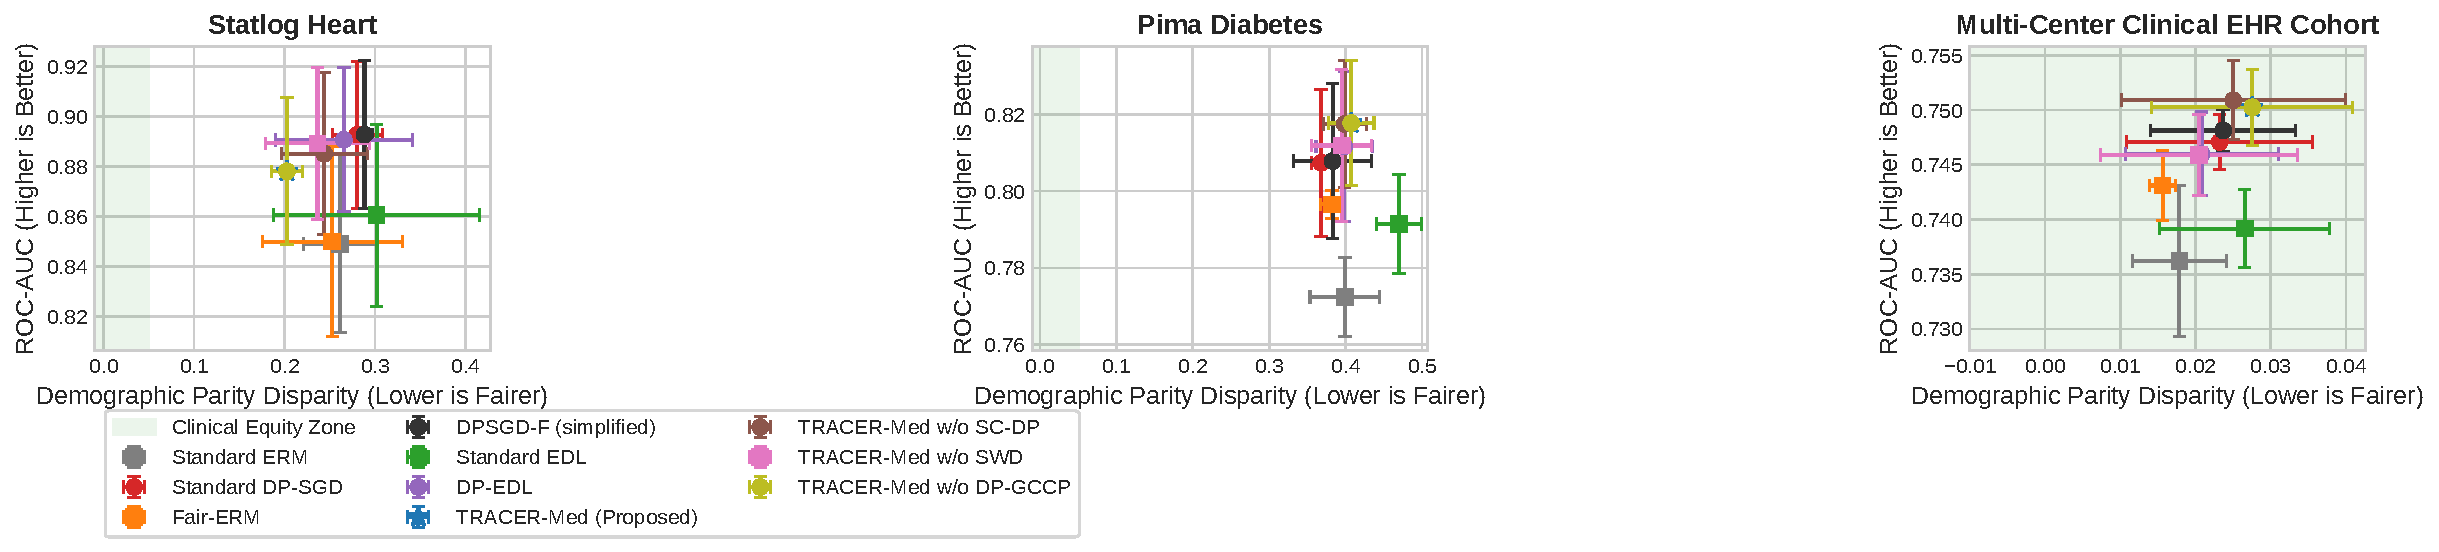
\includegraphics[width=\linewidth]{figures/fig1_utility_vs_fairness.pdf}
\caption{Clinical Utility (ROC-AUC) versus Algorithmic Fairness Disparity ($\Delta_{\text{SP}}$) across all three biomedical benchmarks. ROC-AUC versus statistical parity disparity on the three benchmarks; TRACER-Med has lower parity disparity than the private baselines on Statlog Heart only.}
\label{fig:utility_fairness}
\end{figure*}

\subsection{Conformal Subgroup Coverage and Vacuity}
Figure~\ref{fig:conformal_coverage} shows empirical coverage at nominal miscoverage $\alpha_{\text{conf}} = 0.10$ (target $90\%$). A zero coverage gap is uninformative when every set is $\{0,1\}$, so we report set cardinality alongside the gap and mark vacuous rows ($\bar{|\mathcal{C}|} \ge 1.99$) in Table~\ref{tab:main_results}.
\begin{itemize}
    \item \textbf{Small cohorts.} Private calibration with $\epsilon_{\text{conf}} = 1.0$ on a calibration split of roughly 50 (Heart) to 150 (Pima) records often yields vacuous or nearly vacuous sets. On Pima, DP-SGD has $\bar{|\mathcal{C}|} = 2.00$, TRACER-Med $1.995$, and DP-EDL $1.83$. On Statlog Heart, TRACER-Med has $2.00$, while the private baselines have $1.61$--$1.96$. TRACER-Med is also the worst calibrated model on Heart, and we hypothesize that the prototype anchoring leaves its scores underconfident, so that the private quantile threshold exceeds the scores of both classes. We have not isolated this cause. In the sweep (Table~\ref{tab:sweep}), the TRACER-Med sets on Heart remain vacuous at every noise level.
    \item \textbf{Large cohort.} On the EHR cohort, TRACER-Med gives sets of average size $1.89$, comparable to DP-EDL ($1.90$) and the DPSGD-F-style baseline ($1.89$), and smaller than DP-SGD ($1.94$). Across noise multipliers, its set size ($1.83$--$1.89$) is smaller than that of DP-SGD ($1.92$--$2.00$) and DP-EDL ($1.91$--$1.98$). Its subgroup coverage gap ($0.010$) is larger than those of the baselines ($0.004$--$0.007$).
\end{itemize}
The DP-GCCP shrinkage estimator therefore does not make private conformal prediction informative at these sample sizes in our experiments.

\begin{figure}[t]
\centering
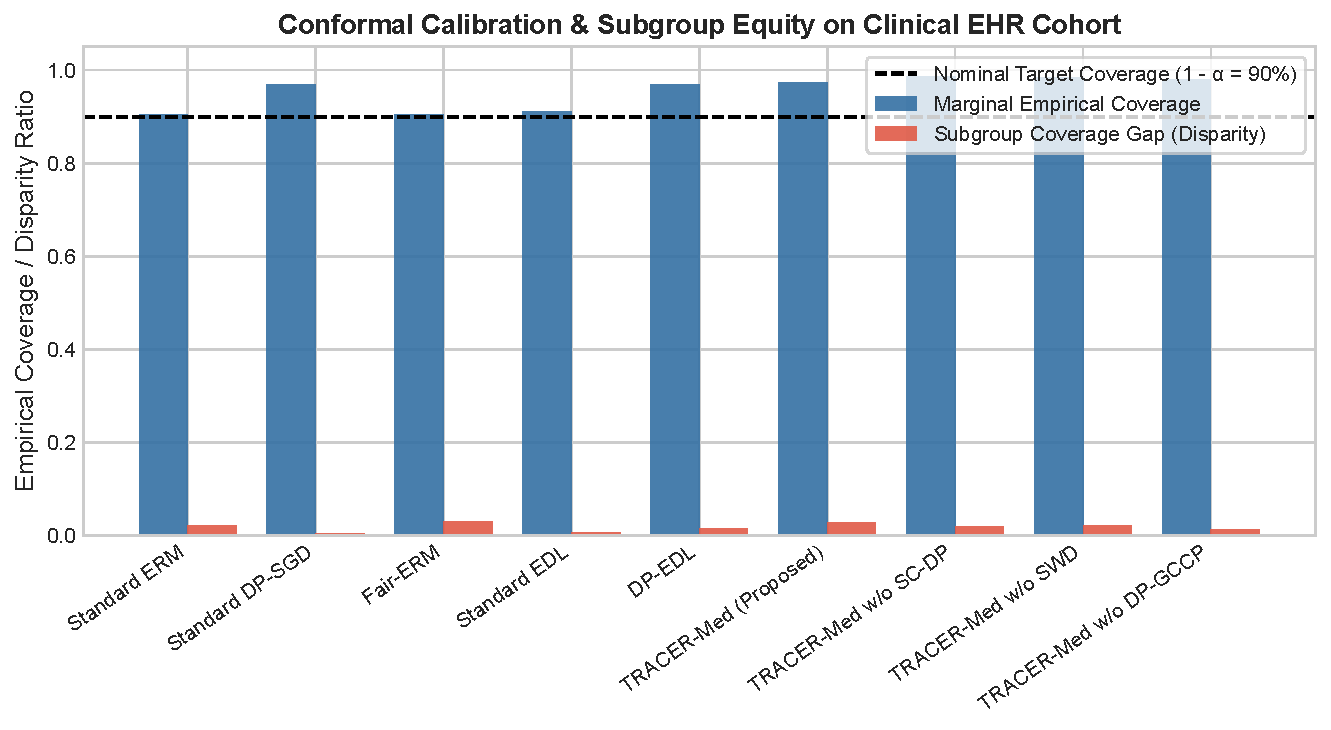
\includegraphics[width=0.88\linewidth]{figures/fig2_conformal_subgroup_coverage.pdf}
\caption{Conformal Calibration and Subgroup Coverage Equity on the Simulated Clinical EHR Cohort at nominal 90\% target coverage. Empirical coverage by demographic group for the evaluated models.}
\label{fig:conformal_coverage}
\end{figure}

\subsection{Empirical Privacy Leakage Auditing}
We audited all models with a loss-threshold membership-inference attack~\cite{shokri2017membership,yeom2018privacy}, following the audit guidance of Carlini et al.~\cite{carlini2022membership}. Non-private models leak noticeably on the small cohorts: MIA AUC is $0.585$--$0.611$ on Statlog Heart and $0.563$--$0.603$ on Pima for ERM, Fair-ERM, and EDL. Private models have MIA AUC between $0.502$ and $0.543$. TRACER-Med has the lowest value among the private models on all three cohorts ($0.516$ on Heart, $0.512$ on Pima, $0.502$ on EHR), and it remains lowest or tied for lowest at every noise level in the sweep, but the margin over the other private models is small (about $0.02$ on the small cohorts and $0.004$ on EHR). Empirical attacks lower-bound vulnerability and do not substitute for the formal guarantee. That guarantee is $(\epsilon, \delta)$-DP with the $\epsilon$ values reported in Section~\ref{sec:experiments} and Section~\ref{sec:sweep}.

\subsection{Noise-Multiplier Sweep}
\label{sec:sweep}
Table~\ref{tab:sweep} varies the noise multiplier from $0.8$ to $3.0$ for DP-SGD, DP-EDL, and TRACER-Med (five splits per cell). On Statlog Heart, the baselines keep ROC-AUC near $0.89$ throughout, while TRACER-Med falls from $0.890$ to $0.734$ ($\epsilon$ from $27.7$ to $4.1$), and its ECE and conformal sets stay worse than DP-EDL's at most noise levels. Its statistical parity disparity stays near $0.24$ against $0.29$--$0.34$ for the baselines. On Pima, ROC-AUC of TRACER-Med is comparable to the baselines up to noise multiplier $2.0$ and lower at $3.0$ ($0.797$ versus $0.823$), and its parity disparity is higher than the baselines' at every level from $1.0$ upward. On the EHR cohort, ROC-AUC and parity disparity are indistinguishable across models, while TRACER-Med has lower ECE at every noise level ($0.055$--$0.088$ versus $0.117$--$0.216$). Equalized Odds and membership-inference results follow the same pattern as in the main table and are in the released CSV.

\begin{table*}[t]
\centering
\small
\caption{Noise-multiplier sweep (mean over five splits): ROC-AUC, statistical parity disparity $\Delta_{\text{SP}}$, and ECE for Standard DP-SGD, DP-EDL, and TRACER-Med. $\epsilon$ at $\delta = 10^{-5}$.}
\label{tab:sweep}
\resizebox{\textwidth}{!}{
\begin{tabular}{llccccccccc}
\toprule
 & & \multicolumn{3}{c}{ROC-AUC $\uparrow$} & \multicolumn{3}{c}{$\Delta_{\text{SP}}$ $\downarrow$} & \multicolumn{3}{c}{ECE $\downarrow$} \\
\cmidrule(lr){3-5}\cmidrule(lr){6-8}\cmidrule(lr){9-11}
$\sigma_{\text{DP}}$ & $\epsilon$ & DP-SGD & DP-EDL & TRACER & DP-SGD & DP-EDL & TRACER & DP-SGD & DP-EDL & TRACER \\
\midrule
\multicolumn{11}{l}{\emph{Benchmark 1: Statlog Heart Disease}} \\
0.8 & 27.7 & 0.901 & 0.897 & 0.890 & 0.312 & 0.325 & 0.243 & 0.142 & 0.080 & 0.169 \\
1.0 & 19.2 & 0.897 & 0.895 & 0.875 & 0.316 & 0.334 & 0.257 & 0.139 & 0.082 & 0.076 \\
1.5 & 10.1 & 0.895 & 0.894 & 0.824 & 0.292 & 0.293 & 0.238 & 0.137 & 0.102 & 0.106 \\
2.0 & 6.8 & 0.895 & 0.894 & 0.787 & 0.323 & 0.341 & 0.242 & 0.127 & 0.119 & 0.128 \\
3.0 & 4.1 & 0.892 & 0.892 & 0.734 & 0.316 & 0.320 & 0.244 & 0.130 & 0.141 & 0.100 \\
\midrule
\multicolumn{11}{l}{\emph{Benchmark 2: Pima Indians Diabetes}} \\
0.8 & 17.5 & 0.825 & 0.828 & 0.831 & 0.385 & 0.412 & 0.399 & 0.190 & 0.105 & 0.141 \\
1.0 & 10.7 & 0.826 & 0.829 & 0.829 & 0.401 & 0.407 & 0.417 & 0.179 & 0.115 & 0.117 \\
1.5 & 5.5 & 0.826 & 0.829 & 0.826 & 0.404 & 0.409 & 0.445 & 0.178 & 0.103 & 0.158 \\
2.0 & 3.7 & 0.826 & 0.828 & 0.820 & 0.401 & 0.386 & 0.465 & 0.171 & 0.082 & 0.132 \\
3.0 & 2.3 & 0.823 & 0.823 & 0.797 & 0.385 & 0.383 & 0.420 & 0.155 & 0.080 & 0.153 \\
\midrule
\multicolumn{11}{l}{\emph{Benchmark 3: Simulated Inpatient EHR Cohort}} \\
0.8 & 7.3 & 0.748 & 0.748 & 0.753 & 0.021 & 0.020 & 0.028 & 0.216 & 0.142 & 0.080 \\
1.0 & 4.4 & 0.748 & 0.748 & 0.752 & 0.020 & 0.021 & 0.027 & 0.213 & 0.137 & 0.072 \\
1.5 & 2.2 & 0.748 & 0.748 & 0.752 & 0.022 & 0.020 & 0.030 & 0.209 & 0.132 & 0.056 \\
2.0 & 1.5 & 0.747 & 0.748 & 0.750 & 0.021 & 0.020 & 0.018 & 0.206 & 0.127 & 0.055 \\
3.0 & 0.9 & 0.746 & 0.748 & 0.747 & 0.018 & 0.020 & 0.026 & 0.202 & 0.117 & 0.088 \\
\bottomrule
\end{tabular}
}
\end{table*}

\subsection{Dual-Channel Dirichlet Attribution (DCDA)}
Figure~\ref{fig:dual_xai} illustrates the attribution patterns generated by our Dual-Channel Dirichlet Attribution mechanism on representative inpatient deterioration episodes.
\begin{itemize}
    \item \textbf{Channel A (Diagnostic Risk Evidence):} Highlights key physiological indicators---elevated lactate ($> 4.0$ mmol/L), hypotension (MAP $< 65$ mmHg / SBP $< 90$ mmHg), and elevated SOFA organ dysfunction scores---as primary positive drivers of clinical deterioration risk. Explanation infidelity of the Dirichlet attributions is reported in Table~\ref{tab:main_results}. It is measured against a different attribution method for the non-evidential baselines, so these values compare the attributions, not the models.
    \item \textbf{Channel B (Epistemic Doubt):} Identifies physiological measurements associated with high Epistemic Mutual Information. In patient presentations with borderline vital signs and ambiguous indicators, Channel B reflects elevated epistemic uncertainty, signaling to the clinician that additional diagnostic testing may be warranted before clinical escalation.
\end{itemize}

\begin{figure*}[t]
\centering
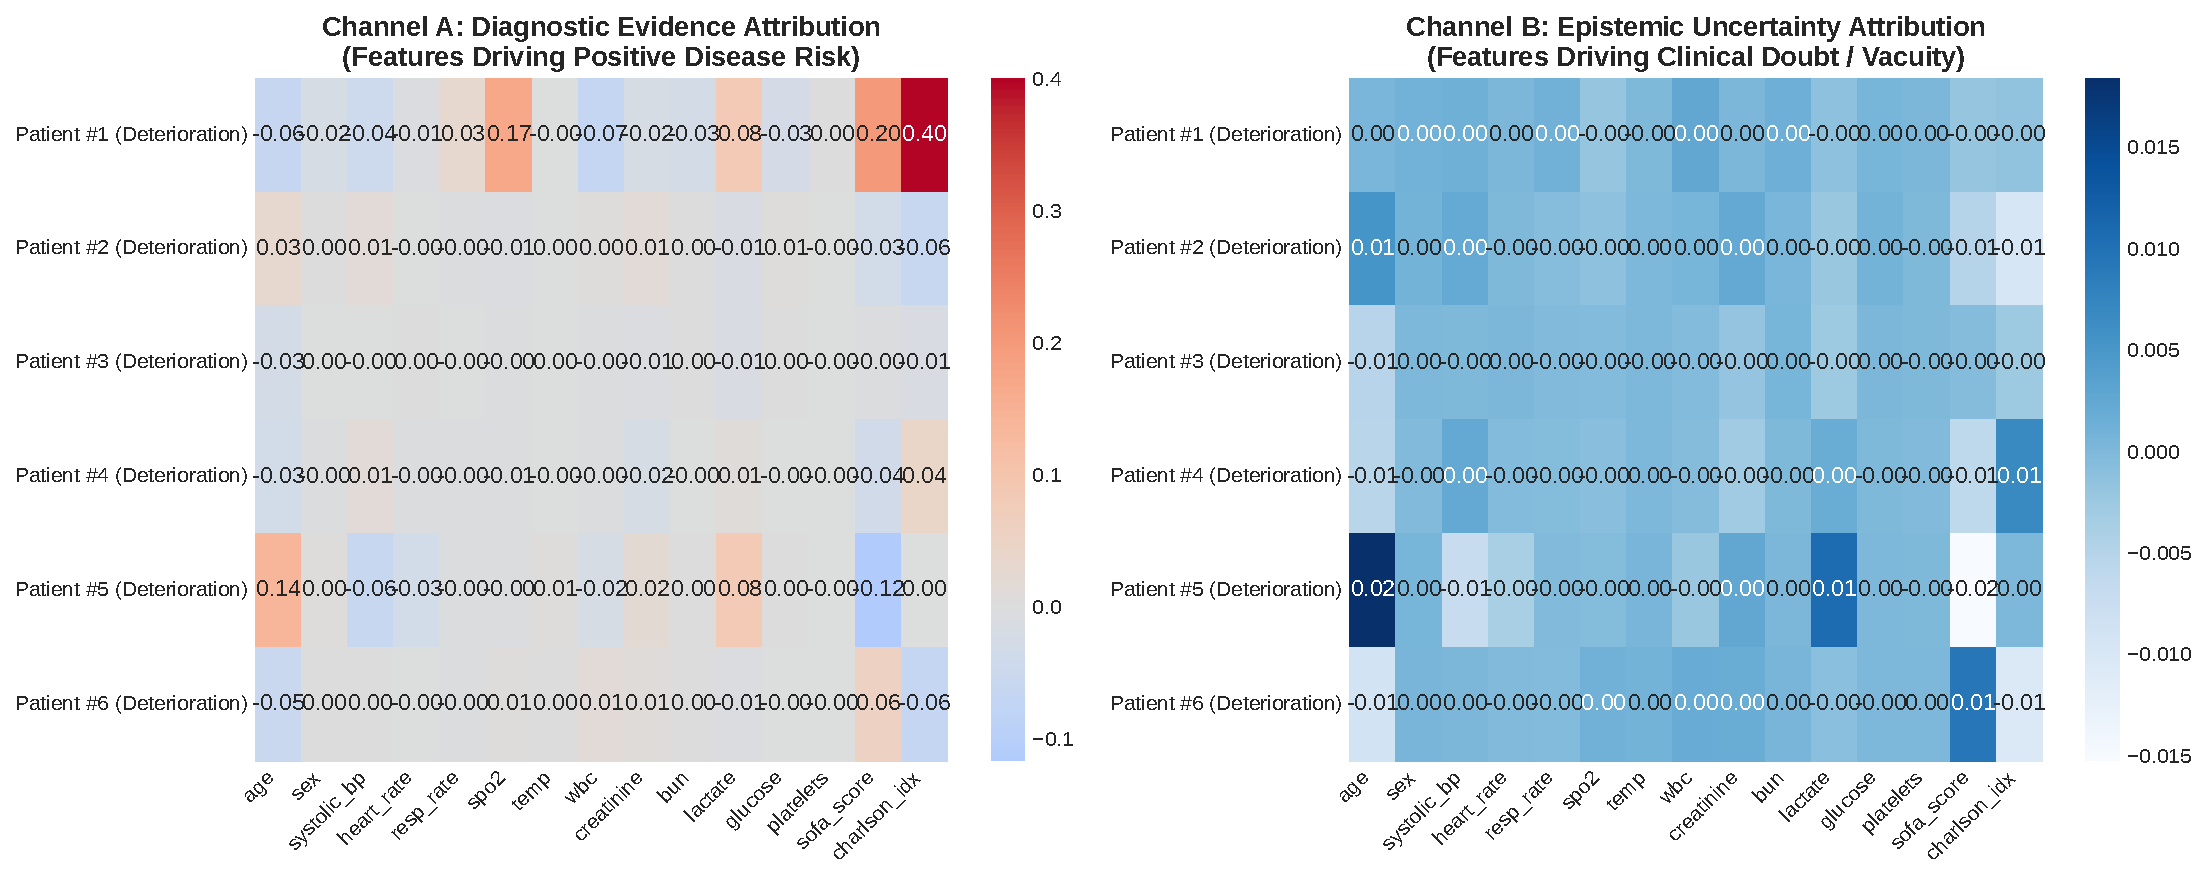
\includegraphics[width=\linewidth]{figures/fig3_dual_channel_attribution.pdf}
\caption{Dual-Channel Dirichlet Attribution (DCDA) heatmaps for illustrative acute clinical deterioration cases. Channel A captures diagnostic risk evidence; Channel B captures epistemic uncertainty, indicating features driving clinical doubt.}
\label{fig:dual_xai}
\end{figure*}

\subsection{Holistic Multi-Pillar Trustworthiness Profile}
Figure~\ref{fig:trustworthiness_radar} illustrates the multi-pillar radar profiles comparing TRACER-Med with baseline paradigms across five core clinical trustworthiness dimensions: diagnostic discrimination (ROC-AUC), calibration (1 - ECE), algorithmic fairness equity (1 - $\Delta_{\text{EO}}$), empirical privacy resistance (1 - MIA AUC), and conformal coverage equity (1 - Cov. Gap). On the EHR cohort the profile of TRACER-Med is close to that of the other private models on most axes, with better calibration. On the smaller cohorts the privacy axis improves slightly while calibration and conformal informativeness do not, so the profile shows a trade-off, not a resolution of the trilemma.

\begin{figure}[t]
\centering
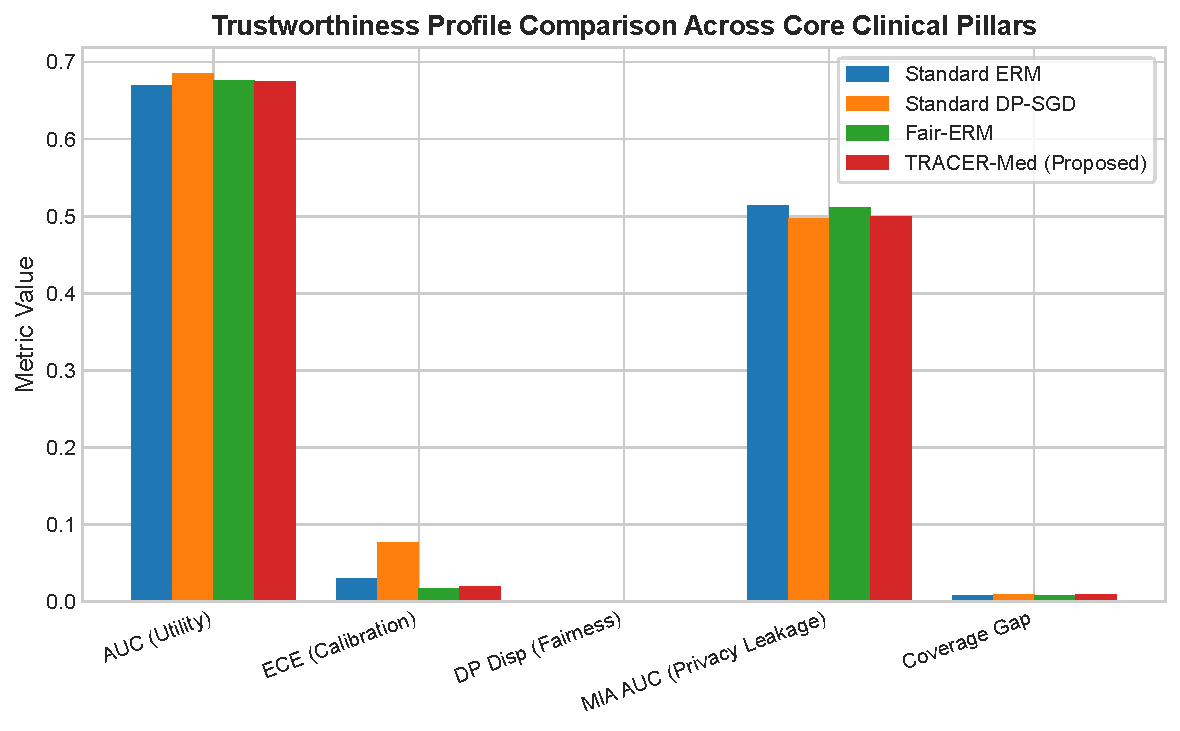
\includegraphics[width=0.92\linewidth]{figures/fig4_trustworthiness_profile.pdf}
\caption{Multi-pillar Trustworthiness Profile across clinical utility (ROC-AUC), calibration (1 - ECE), equalized odds equity (1 - $\Delta_{\text{EO}}$), empirical privacy resistance (1 - MIA AUC), and conformal coverage equity (1 - Cov. Gap). Comparison of TRACER-Med with ERM, DP-SGD, and Fair-ERM.}
\label{fig:trustworthiness_radar}
\end{figure}

\subsection{Ablation Studies}
Table~\ref{tab:ablation} removes one module at a time on the same three splits.
\begin{enumerate}
    \item \emph{Removing prototype alignment (w/o PC-PAT).} On Heart, $\Delta_{\text{SP}}$ rises from $0.203$ to $0.236$ and $\Delta_{\text{EO}}$ falls from $0.110$ to $0.078$, while ECE falls from $0.195$ to $0.072$ and the conformal sets stop being vacuous ($1.96$). On Pima and EHR the changes in disparity are within one standard deviation. On EHR, removing the alignment raises ECE from $0.086$ to $0.144$. The alignment term therefore trades calibration and set informativeness against statistical parity on the smallest cohort, and helps calibration on the largest.
    \item \emph{Removing subgroup-calibrated clipping (w/o REF-DP).} Uniform clipping gives $\Delta_{\text{SP}}$ $0.244$ versus $0.203$ on Heart, $0.399$ versus $0.407$ on Pima, and $0.025$ versus $0.028$ on EHR, and $\Delta_{\text{EO}}$ $0.074$ versus $0.110$ on Heart and $0.046$ versus $0.038$ on EHR. All differences are within about one standard deviation. We therefore find no measurable benefit of REF-DP's group-specific thresholds, and the motivation (preventing minority gradient truncation) is not supported by the benchmarks used here. The group weights in our implementation use fixed prior evidence strengths, not strengths estimated from the Dirichlet Fisher metric during training, which may understate the method.
    \item \emph{Removing group-conditional conformal calibration (w/o DP-GCCP).} Heart and EHR results are identical to the full model, and on Pima the average set size falls from $1.995$ to $1.75$ at the cost of a coverage gap of $0.009$. We cannot attribute informative sets to the group-conditional mechanism at these sample sizes.
\end{enumerate}

\begin{table}[t]
\centering
\caption{Ablation analysis on all three benchmarks (mean $\pm$ std over 3 random splits). Bold marks the best value within each benchmark among the four configurations; $^*$vacuous conformal sets (cardinality $\ge 1.99$) are not bolded.}
\label{tab:ablation}
\resizebox{\linewidth}{!}{
\begin{tabular}{lcccccc}
\toprule
\textbf{Configuration} & \textbf{ROC-AUC} $\uparrow$ & \textbf{ECE} $\downarrow$ & $\Delta_{\text{SP}}$ $\downarrow$ & $\Delta_{\text{EO}}$ $\downarrow$ & \textbf{Cov. Gap} $\downarrow$ & \textbf{Set Size} $\downarrow$ \\
\midrule
\multicolumn{7}{l}{\emph{Benchmark 1: Statlog Heart Disease}} \\
\textbf{TRACER-Med (Full)} & $0.878 \pm 0.029$ & $0.195 \pm 0.045$ & $\mathbf{0.203} \pm \mathbf{0.017}$ & $0.110 \pm 0.077$ & $0.000 \pm 0.000^*$ & $2.00 \pm 0.00^*$ \\
\quad w/o REF-DP (uniform clipping) & $0.885 \pm 0.032$ & $0.194 \pm 0.028$ & $0.244 \pm 0.048$ & $\mathbf{0.074} \pm \mathbf{0.008}$ & $0.000 \pm 0.000^*$ & $2.00 \pm 0.00^*$ \\
\quad w/o PC-PAT (no prototype alignment) & $\mathbf{0.889} \pm \mathbf{0.030}$ & $\mathbf{0.072} \pm \mathbf{0.011}$ & $0.236 \pm 0.057$ & $0.078 \pm 0.007$ & $\mathbf{0.007} \pm \mathbf{0.010}$ & $1.96 \pm 0.06$ \\
\quad w/o DP-GCCP (marginal CP) & $0.878 \pm 0.029$ & $0.195 \pm 0.045$ & $\mathbf{0.203} \pm \mathbf{0.017}$ & $0.110 \pm 0.077$ & $0.000 \pm 0.000^*$ & $2.00 \pm 0.00^*$ \\
\midrule
\multicolumn{7}{l}{\emph{Benchmark 2: Pima Indians Diabetes}} \\
\textbf{TRACER-Med (Full)} & $\mathbf{0.818} \pm \mathbf{0.016}$ & $0.130 \pm 0.005$ & $0.407 \pm 0.030$ & $0.278 \pm 0.050$ & $0.000 \pm 0.000^*$ & $1.99 \pm 0.01^*$ \\
\quad w/o REF-DP (uniform clipping) & $0.818 \pm 0.016$ & $0.134 \pm 0.006$ & $0.399 \pm 0.028$ & $0.272 \pm 0.050$ & $\mathbf{0.000} \pm \mathbf{0.000}$ & $1.98 \pm 0.03$ \\
\quad w/o PC-PAT (no prototype alignment) & $0.812 \pm 0.020$ & $\mathbf{0.118} \pm \mathbf{0.005}$ & $\mathbf{0.395} \pm \mathbf{0.039}$ & $\mathbf{0.264} \pm \mathbf{0.050}$ & $0.000 \pm 0.000^*$ & $2.00 \pm 0.00^*$ \\
\quad w/o DP-GCCP (marginal CP) & $\mathbf{0.818} \pm \mathbf{0.016}$ & $0.130 \pm 0.005$ & $0.407 \pm 0.030$ & $0.278 \pm 0.050$ & $0.009 \pm 0.007$ & $1.75 \pm 0.02$ \\
\midrule
\multicolumn{7}{l}{\emph{Benchmark 3: Simulated Inpatient EHR Cohort}} \\
\textbf{TRACER-Med (Full)} & $0.750 \pm 0.003$ & $\mathbf{0.086} \pm \mathbf{0.007}$ & $0.028 \pm 0.013$ & $\mathbf{0.038} \pm \mathbf{0.028}$ & $0.010 \pm 0.005$ & $1.89 \pm 0.04$ \\
\quad w/o REF-DP (uniform clipping) & $\mathbf{0.751} \pm \mathbf{0.004}$ & $0.096 \pm 0.005$ & $0.025 \pm 0.015$ & $0.046 \pm 0.027$ & $\mathbf{0.010} \pm \mathbf{0.007}$ & $1.90 \pm 0.07$ \\
\quad w/o PC-PAT (no prototype alignment) & $0.746 \pm 0.004$ & $0.144 \pm 0.003$ & $\mathbf{0.020} \pm \mathbf{0.013}$ & $0.045 \pm 0.023$ & $0.012 \pm 0.011$ & $1.93 \pm 0.05$ \\
\quad w/o DP-GCCP (marginal CP) & $0.750 \pm 0.003$ & $\mathbf{0.086} \pm \mathbf{0.007}$ & $0.028 \pm 0.013$ & $\mathbf{0.038} \pm \mathbf{0.028}$ & $0.010 \pm 0.005$ & $1.89 \pm 0.04$ \\
\bottomrule
\end{tabular}
}
\end{table}

\section{Clinical Governance, Deployment, and Regulatory Alignment}
\label{sec:governance}

\subsection{Regulatory Alignment (FDA GMLP, PCCP, HHS, EU AI Act)}
Regulatory frameworks increasingly mandate comprehensive documentation and formal risk controls for clinical AI algorithms. TRACER-Med is designed to support the technical documentation required under international regulatory guidelines:
\begin{itemize}
    \item \textbf{FDA Good Machine Learning Practice (GMLP):} The U.S. FDA, Health Canada, and UK MHRA established 10 Guiding Principles for GMLP in medical device development~\cite{fda2021gmlp}. TRACER-Med supports Principle 3 (addressing training data representativeness and subgroup gradient balance via REF-DP and PC-PAT), Principle 6 (tailored model design separating aleatoric from epistemic uncertainty), Principle 7 (focusing on human-AI clinical team performance via dual-channel risk and doubt attributions), and Principle 9 (providing clear, contextually relevant information through distribution-free conformal safety bounds and uncertainty metrics).
    \item \textbf{FDA Predetermined Change Control Plans (PCCP):} Under the FDA's finalized guidance on Predetermined Change Control Plans for AI-Enabled Device Software Functions (issued December 2024~\cite{fda2024pccp}), manufacturers must specify predetermined modification protocols for post-market model updates. TRACER-Med's formal Differential Privacy parameters $(\epsilon, \delta)$ and distribution-free conformal calibration bounds establish quantifiable guardrails for model retraining, while accounting for privacy loss accumulation across release cycles.
    \item \textbf{EU AI Act and HHS Section 1557:} Under the European Union Artificial Intelligence Act (Regulation (EU) 2024/1689~\cite{euaiact2024}), medical diagnostic AI systems classified as High-Risk AI Systems under Annex I (governed by MDR/IVDR) are subject to technical verification of risk management (Article 9), data governance (Article 10), technical documentation (Article 11), record-keeping (Article 12), transparency (Article 13), human oversight (Article 14), and accuracy/robustness (Article 15). In parallel, U.S. HHS Section 1557 rules (45 CFR §92.210) prohibit discriminatory algorithmic practices in healthcare programs. TRACER-Med supports technical documentation by quantifying demographic error disparity (for example $\Delta_{\text{EO}} = 0.110$ on cardiovascular data and $0.278$ on metabolic data, which are not lower than those of the baselines), enabling auditable clinical equity reviews.
\end{itemize}

\subsection{Clinical Workflow Integration and Selective Abstention}
In practical clinical environments, TRACER-Med can be structured as an augmented decision-support co-pilot:
\begin{enumerate}
    \item When a patient profile yields a singleton prediction set $\mathcal{C}(\mathbf{x}) = \{k\}$ accompanied by low relative vacuity ($u \le u_{\text{thresh}}$, calibrated to the lower tertile of validation cohort evidence where total evidence $S \ge 4.0$), the system provides a high-confidence diagnostic alert supported by Channel A biomarker attributions.
    \item When the prediction set is indeterminate ($\mathcal{C}(\mathbf{x}) = \{0, 1\}$) or epistemic uncertainty is elevated ($u > u_{\text{thresh}}$), the system abstains from automated recommendations, routing the case to clinician review while presenting Channel B uncertainty attributions to identify ambiguous or missing physiological parameters.
\end{enumerate}

\subsection{Limitations and Future Work}
Several important limitations should be acknowledged:
\begin{itemize}
    \item \emph{Inference-Time Demographic Requirement:} Group-conditional conformal prediction requires sensitive attribute $A$ at test time to select the cohort-specific threshold $\hat{q}_a$. While demographic covariates are standard in clinical EHR charts, future work should explore group-oblivious conformal procedures.
    \item \emph{Privacy Budgets:} With noise multiplier $0.8$ the exact accountant gives $\epsilon = 27.7$ (Heart), $17.5$ (Pima), and $7.3$ (EHR); the sweep reaches $\epsilon = 4.1$, $2.3$, and $0.9$ at noise multiplier $3.0$. Budgets above roughly $10$ do not provide meaningful protection against a strong adversary.
    \item \emph{Utility Under Heavy Noise on Small Cohorts:} On Statlog Heart, the ROC-AUC of TRACER-Med falls from $0.890$ to $0.734$ as the noise multiplier increases from $0.8$ to $3.0$, whereas the baselines stay near $0.89$.
    \item \emph{Private Conformal Prediction on Small Cohorts:} DP-GCCP gave vacuous or nearly vacuous sets on the two small cohorts at $\epsilon_{\text{conf}} = 1.0$.
    \item \emph{No Equalized Odds Gain and Unsupported REF-DP:} We observed no reduction in Equalized Odds disparity and no measurable benefit of group-specific clipping thresholds.
    \item \emph{Approximate Baseline:} The DPSGD-F-style baseline is our simplified reimplementation with unprivatized threshold statistics. Fair private empirical risk minimization~\cite{tran2021differentially} was not run.
    \item \emph{Unaudited Theory:} The proofs were not independently verified in this revision, and the implementation of REF-DP uses fixed priors, not the Fisher-metric quantities of the derivation.
    \item \emph{Binary Demographic Attributes:} The present formulation focuses on binary sensitive attributes ($a \in \{0, 1\}$). Extending REF-DP and DP-GCCP to continuous attributes or multi-attribute intersections (e.g., age $\times$ sex $\times$ race) requires multi-dimensional quantile estimation.
    \item \emph{Longitudinal Dynamics:} While the current study evaluates static clinical episodes, future research should integrate recurrent or state-space models to capture longitudinal ICU time series.
    \item \emph{Synthetic Cohort Validation:} Although the 10,000-patient EHR cohort was parameterized from realistic MIMIC-IV and eICU distributions, prospective validation on fully credentialed multi-center clinical registries remains an essential next step.
\end{itemize}

\section{Conclusion}
\label{sec:conclusion}
Deploying trustworthy artificial intelligence in healthcare requires balancing the tensions between patient data privacy, demographic fairness, uncertainty quantification, and explainability. We presented \textbf{TRACER-Med}, an integrated deep learning framework addressing the Privacy--Fairness--Uncertainty Trilemma. By combining Evidential Dirichlet Deep Learning, Riemannian Evidential-Fisher Subgroup-Calibrated DP-SGD, class-conditional prototypical anchor representation alignment, Differentially Private Group-Conditional Conformal Prediction, and Dual-Channel Dirichlet Attribution, In experiments on three cohorts with an exact privacy accountant and a common operating point, TRACER-Med has the lowest empirical membership-inference AUC among private models, better calibration on the large simulated cohort across noise levels, and lower statistical parity disparity on Statlog Heart. It does not reduce Equalized Odds disparity, its private conformal layer is uninformative on the two small cohorts, its calibration and utility under heavy noise are worse on Statlog Heart, and subgroup-calibrated clipping shows no measurable benefit. These results motivate study on larger real-world cohorts, on conformal procedures that remain informative under privacy, and on fairness terms that do not trade away calibration.

\section*{Ethics Statement}
This investigation utilized publicly accessible, fully de-identified benchmark datasets (Statlog Heart Disease, OpenML ID: 53; Pima Indians Diabetes, OpenML ID: 37) and a synthetic electronic health record cohort derived from statistical distributions of the MIMIC-IV and eICU repositories without including protected health information. In accordance with institutional policies and national guidelines (45 CFR 46.102), this secondary analysis of de-identified open-source data does not constitute human subjects research and IRB review was not required. Furthermore, we explicitly acknowledge the historical and tribal data governance considerations surrounding the Pima Indians Diabetes dataset, underscoring the importance of Indigenous data sovereignty and respectful secondary analysis.

\section*{CRediT Authorship Contribution Statement}
\textbf{Quang-Vinh Dang:} Conceptualization, Methodology, Software, Validation, Formal analysis, Investigation, Data curation, Writing -- original draft, Writing -- review \& editing, Visualization, Project administration.

\section*{Funding}
This research did not receive any specific grant from funding agencies in the public, commercial, or not-for-profit sectors.

\section*{Declaration of Competing Interests}
The author declares that they have no known competing financial interests or personal relationships that could have appeared to influence the work reported in this paper.

\section*{Data and Code Availability}
The source code, benchmark preparation scripts, synthetic data generation pipelines, and pre-trained evaluation checkpoints are available in the GitHub repository: \url{https://github.com/vinhqdang/biomedical_privacy_research}. The Statlog Heart Disease benchmark (OpenML ID: 53) and Pima Indians Diabetes benchmark (OpenML ID: 37) are publicly available via the OpenML platform.

\section*{Declaration of Generative AI in Scientific Writing}
During the preparation of this work, the author used Claude 3.7 Sonnet (Anthropic) and Google Antigravity in order to assist with manuscript typesetting, literature cross-referencing, and stylistic polishing. After using this tool/service, the author reviewed and edited the content as needed and takes full responsibility for the content of the publication.

\bibliographystyle{elsarticle-num}
\bibliography{references}

\end{document}

